\section{LQR и фильтр Калмана}
\subsection{Линейно-квадратичный регулятор}
Рассмотрим синтез линейно-квадратичного регулятора, минимизирующего функционал качества 
\begin{eqnarray}
J = \int_{0}^{\infty} \left( x^T Q x + u^T R u \right) dt
\end{eqnarray}
где $Q$, $R$ --- матрицы весов.

Решив уравнение Риккати при $v = 1$, получем регулятор:
\begin{equation}
    \begin{cases}
        A^T + PA + Q - vPBR^{-1}B^TP = 0 \\ 
        K = -R^{-1}B^TP
    \end{cases}
\end{equation}
Решение данного уравнения существует при условии, что пара $(A, B)$ является стабилизируемой, 
пара $(Q, A)$ является наблюдаемой. 

Синтезируем регулятор для весовых матриц 
\begin{equation}
    Q = 30 \cdot I_{4\times 4}, \quad R = 1
\end{equation}
\begin{equation}
    K = \begin{bmatrix}
        5.48  & 56.48  & -5414.73  & -1223.92 \\ 
    \end{bmatrix}, \quad J = 33118.54
\end{equation}

Проверим работу полученного регулятора, проведя моделирование системы с начальным углом 
отклонения маятника $\theta_0 = 0.2$. Результат моделирования представлен на рисунке \ref{fig:lqr_controller} и 
\ref{fig:lqr_controller_u} 
\begin{figure}[ht!]
    \centering
    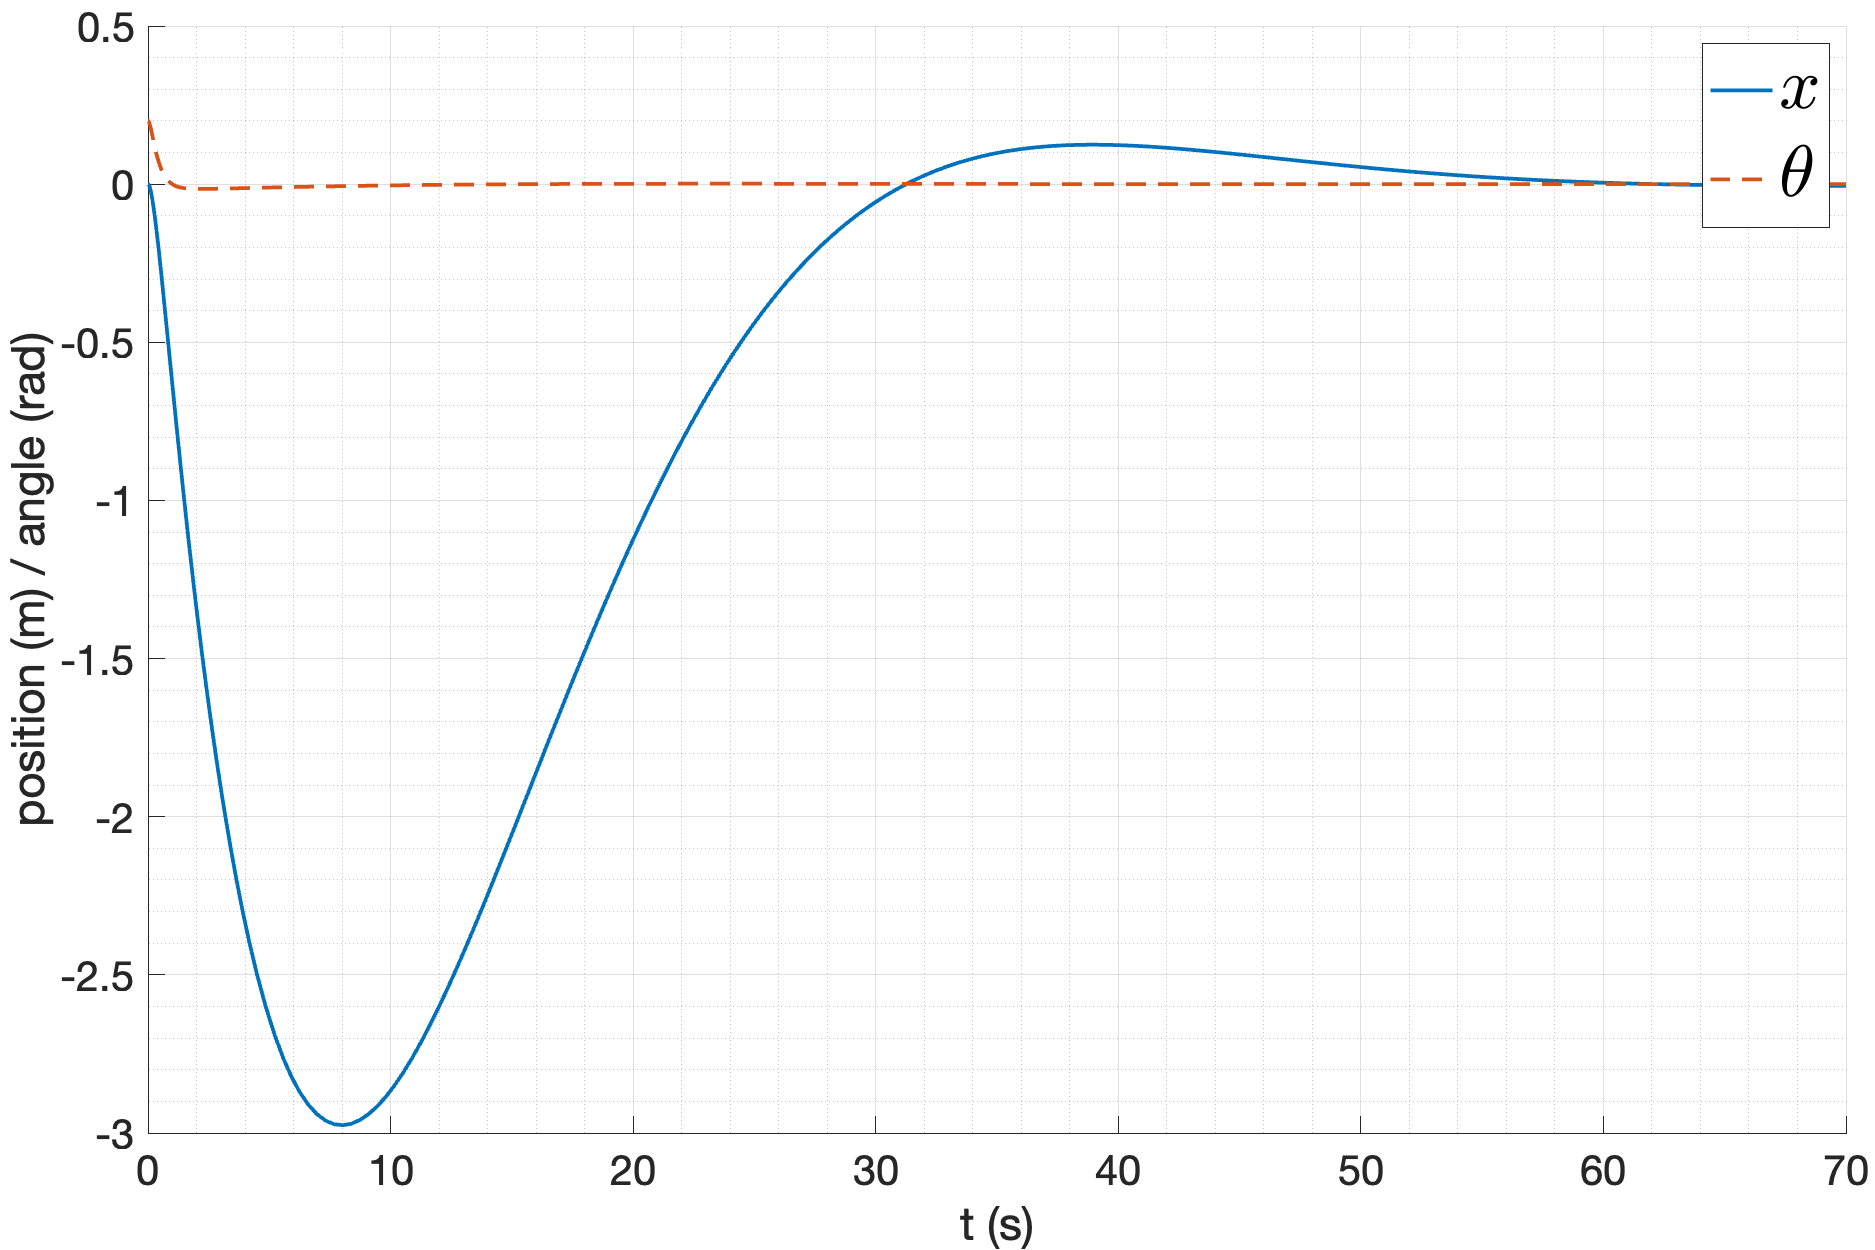
\includegraphics[width=\textwidth]{media/plots/LQR/out_1.png}
    \caption{Результат моделирования системы}
    \label{fig:lqr_controller}
\end{figure}
\begin{figure}[ht!]
    \centering
    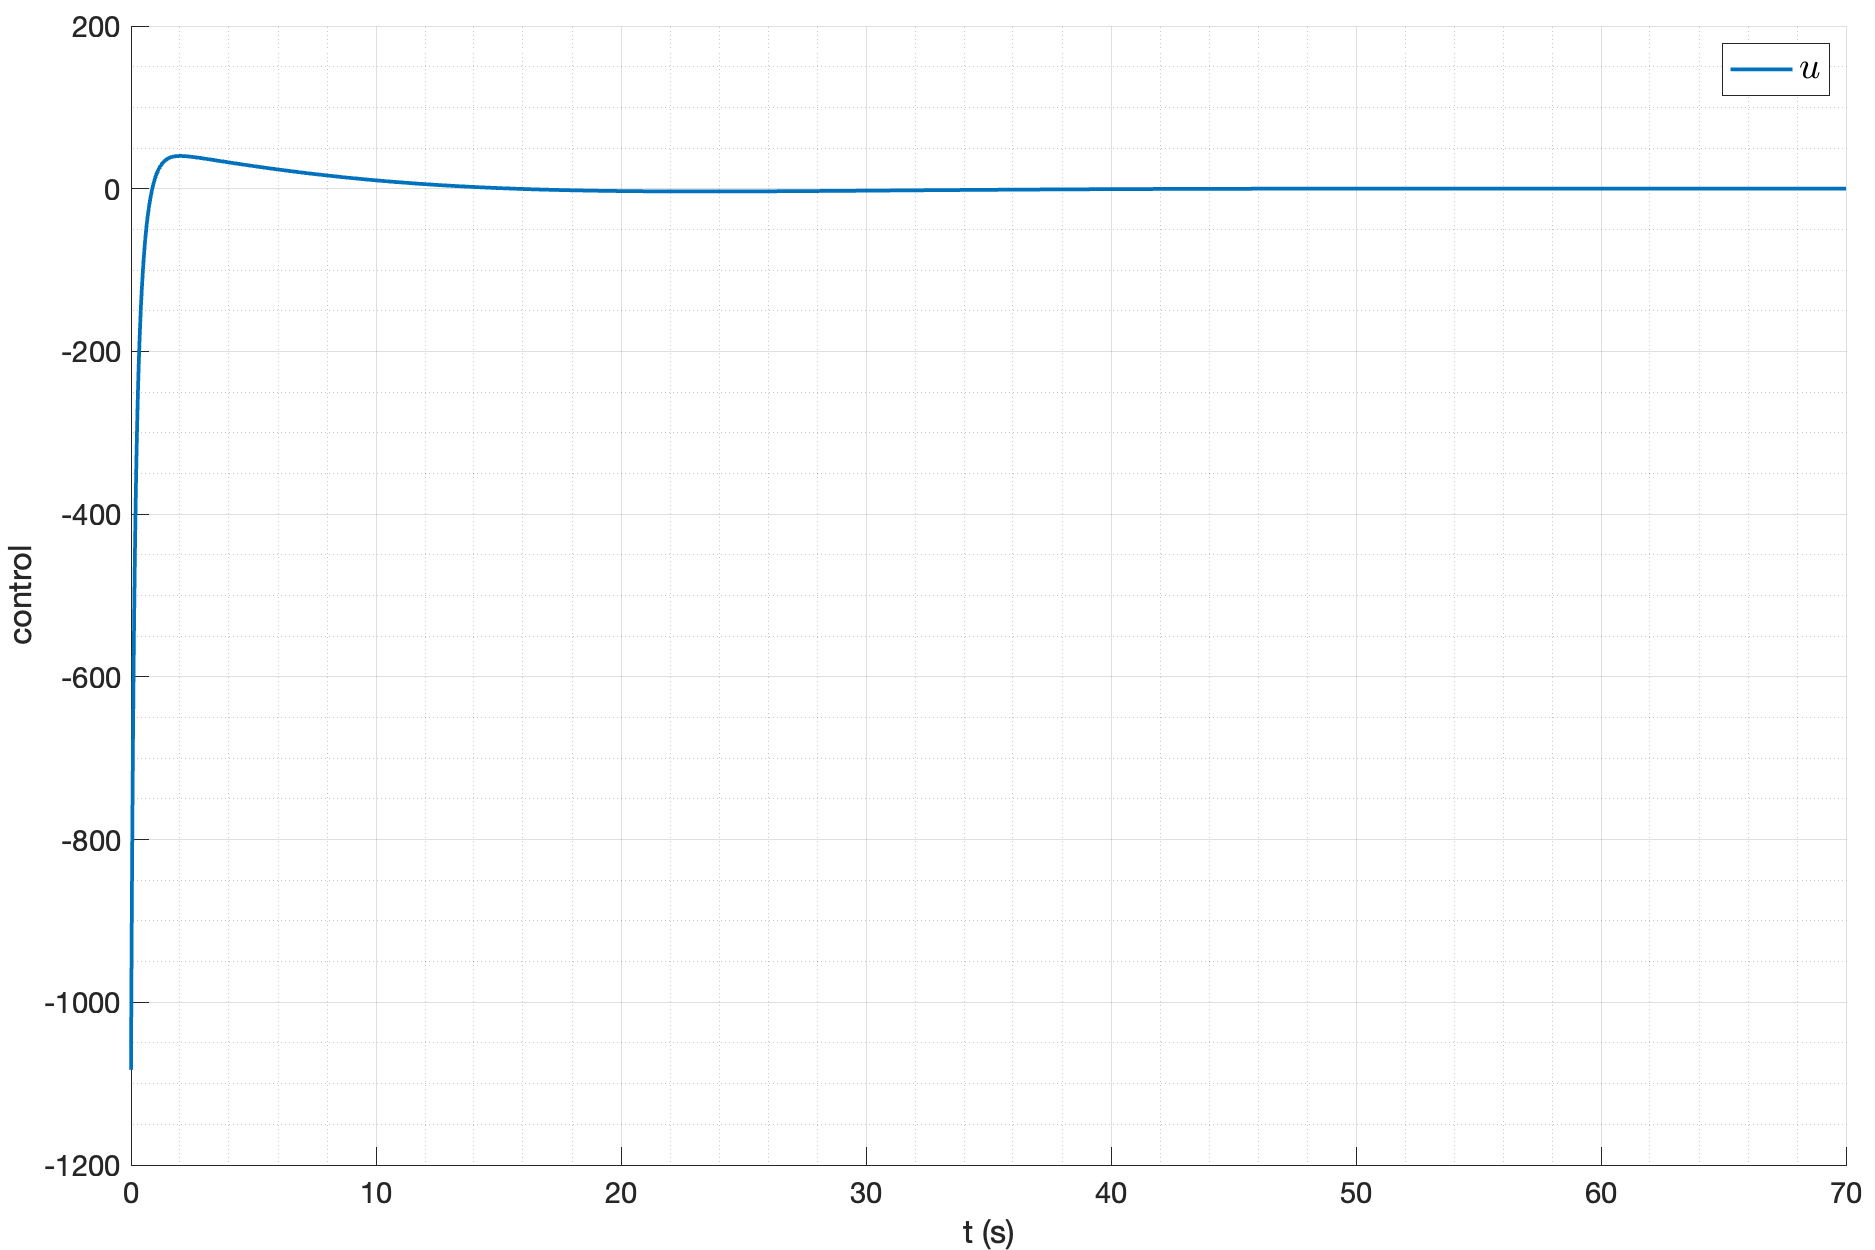
\includegraphics[width=\textwidth]{media/plots/LQR/u_1.png}
    \caption{Управляющее воздействие регулятора}
    \label{fig:lqr_controller_u}
\end{figure}
Видно, что выход системы сходится к нулю, при этом время сходимости угла отклонения маятника сильно 
меньше, чем время сходимости положения тележки. 

\subsection{Исследование устойчивости}
Проверим работу регулятора при различных начальных условиях. Будем рассматривать начальное отклонение 
маятника из множества $\theta_0 \in \begin{bmatrix}0.3 & 0.5 & 1.2 & 1.5\end{bmatrix}$. 
Результаты моделирования представлены на рисунке \ref{fig:lqr_controller_2}.
\begin{figure}[ht!]
    \centering
    \begin{subfigure}[b]{0.45\textwidth}
        \centering
        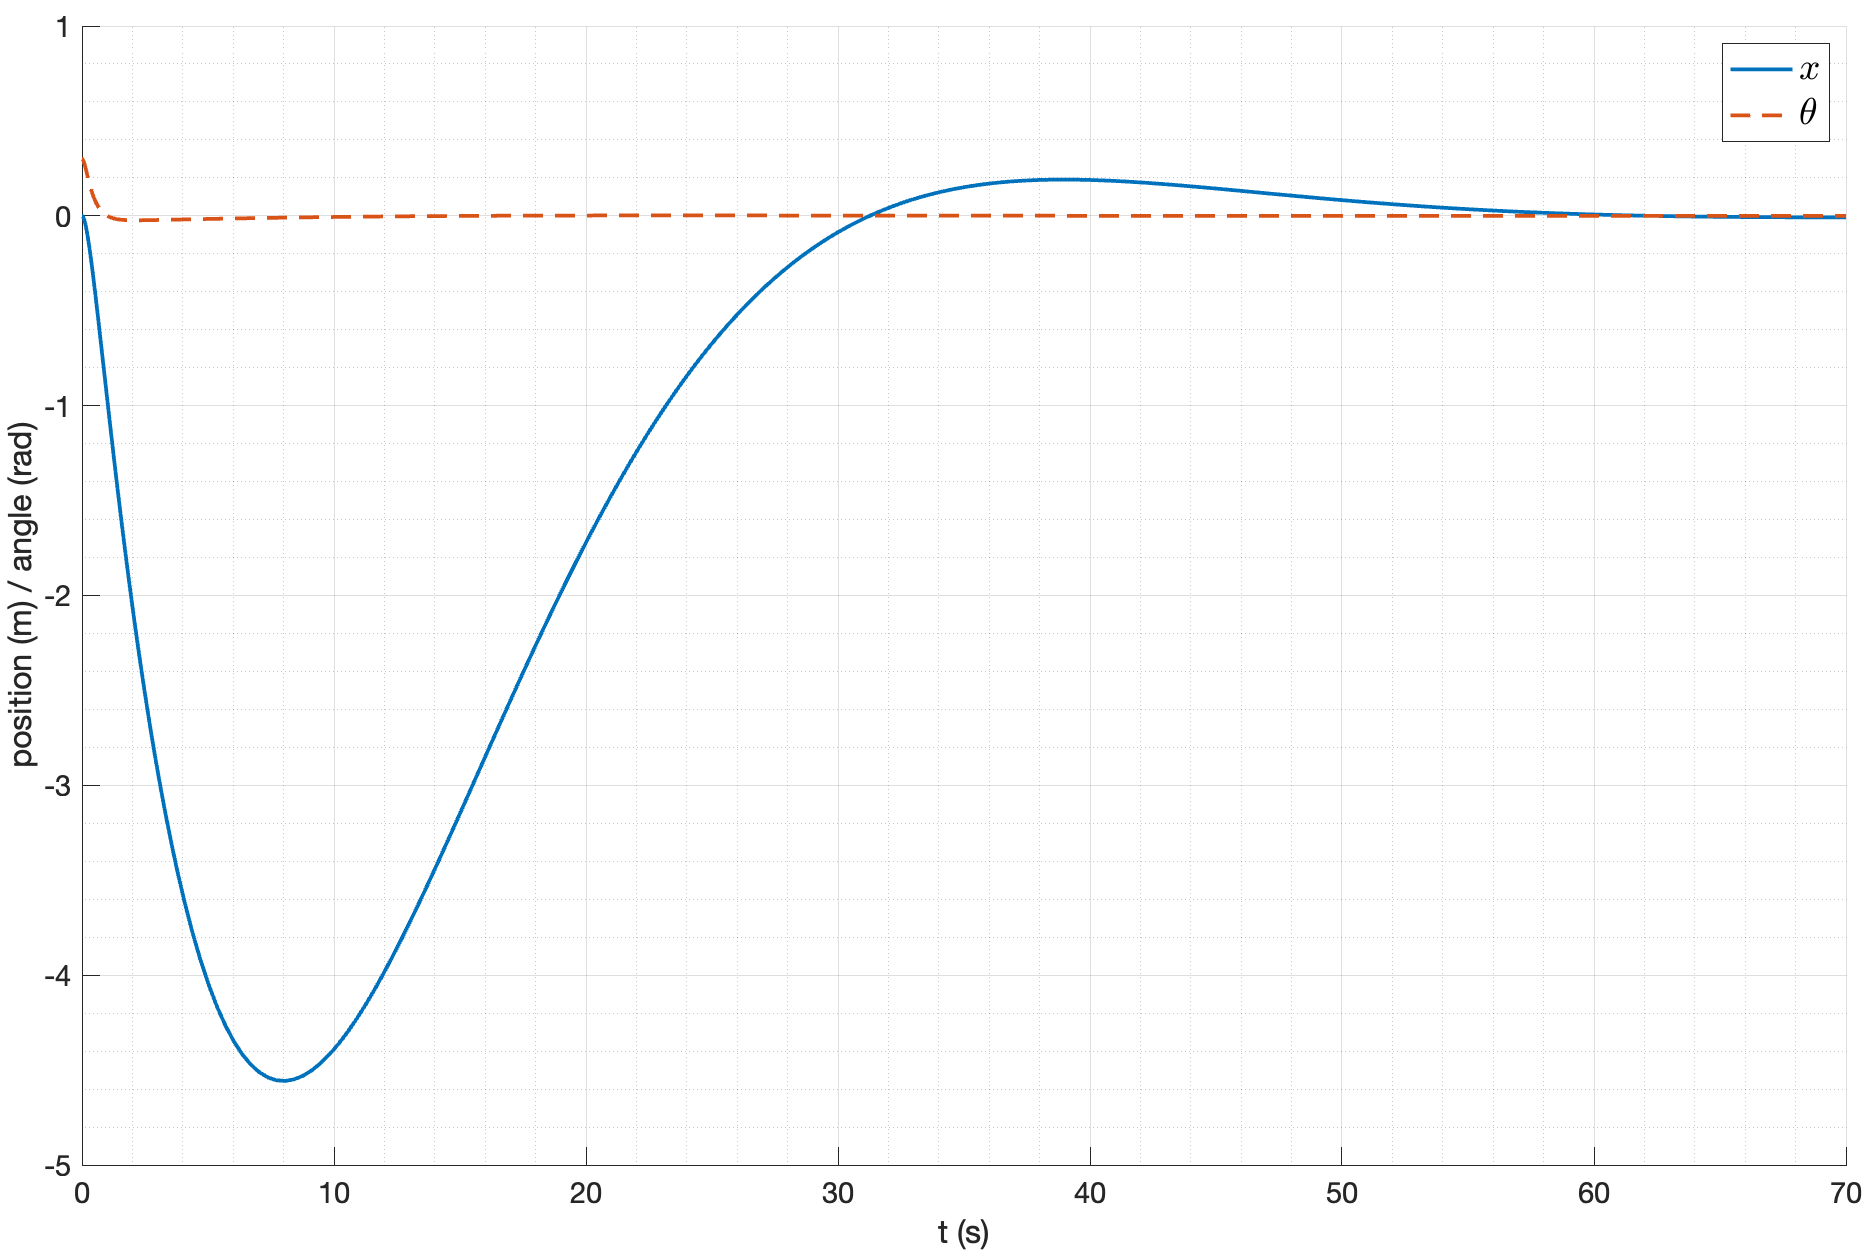
\includegraphics[width=\textwidth]{media/plots/LQR/out_2.png}
        \caption{Результат моделирования при $\theta_0 = 0.3$}
    \end{subfigure}
    \begin{subfigure}[b]{0.45\textwidth}
        \centering
        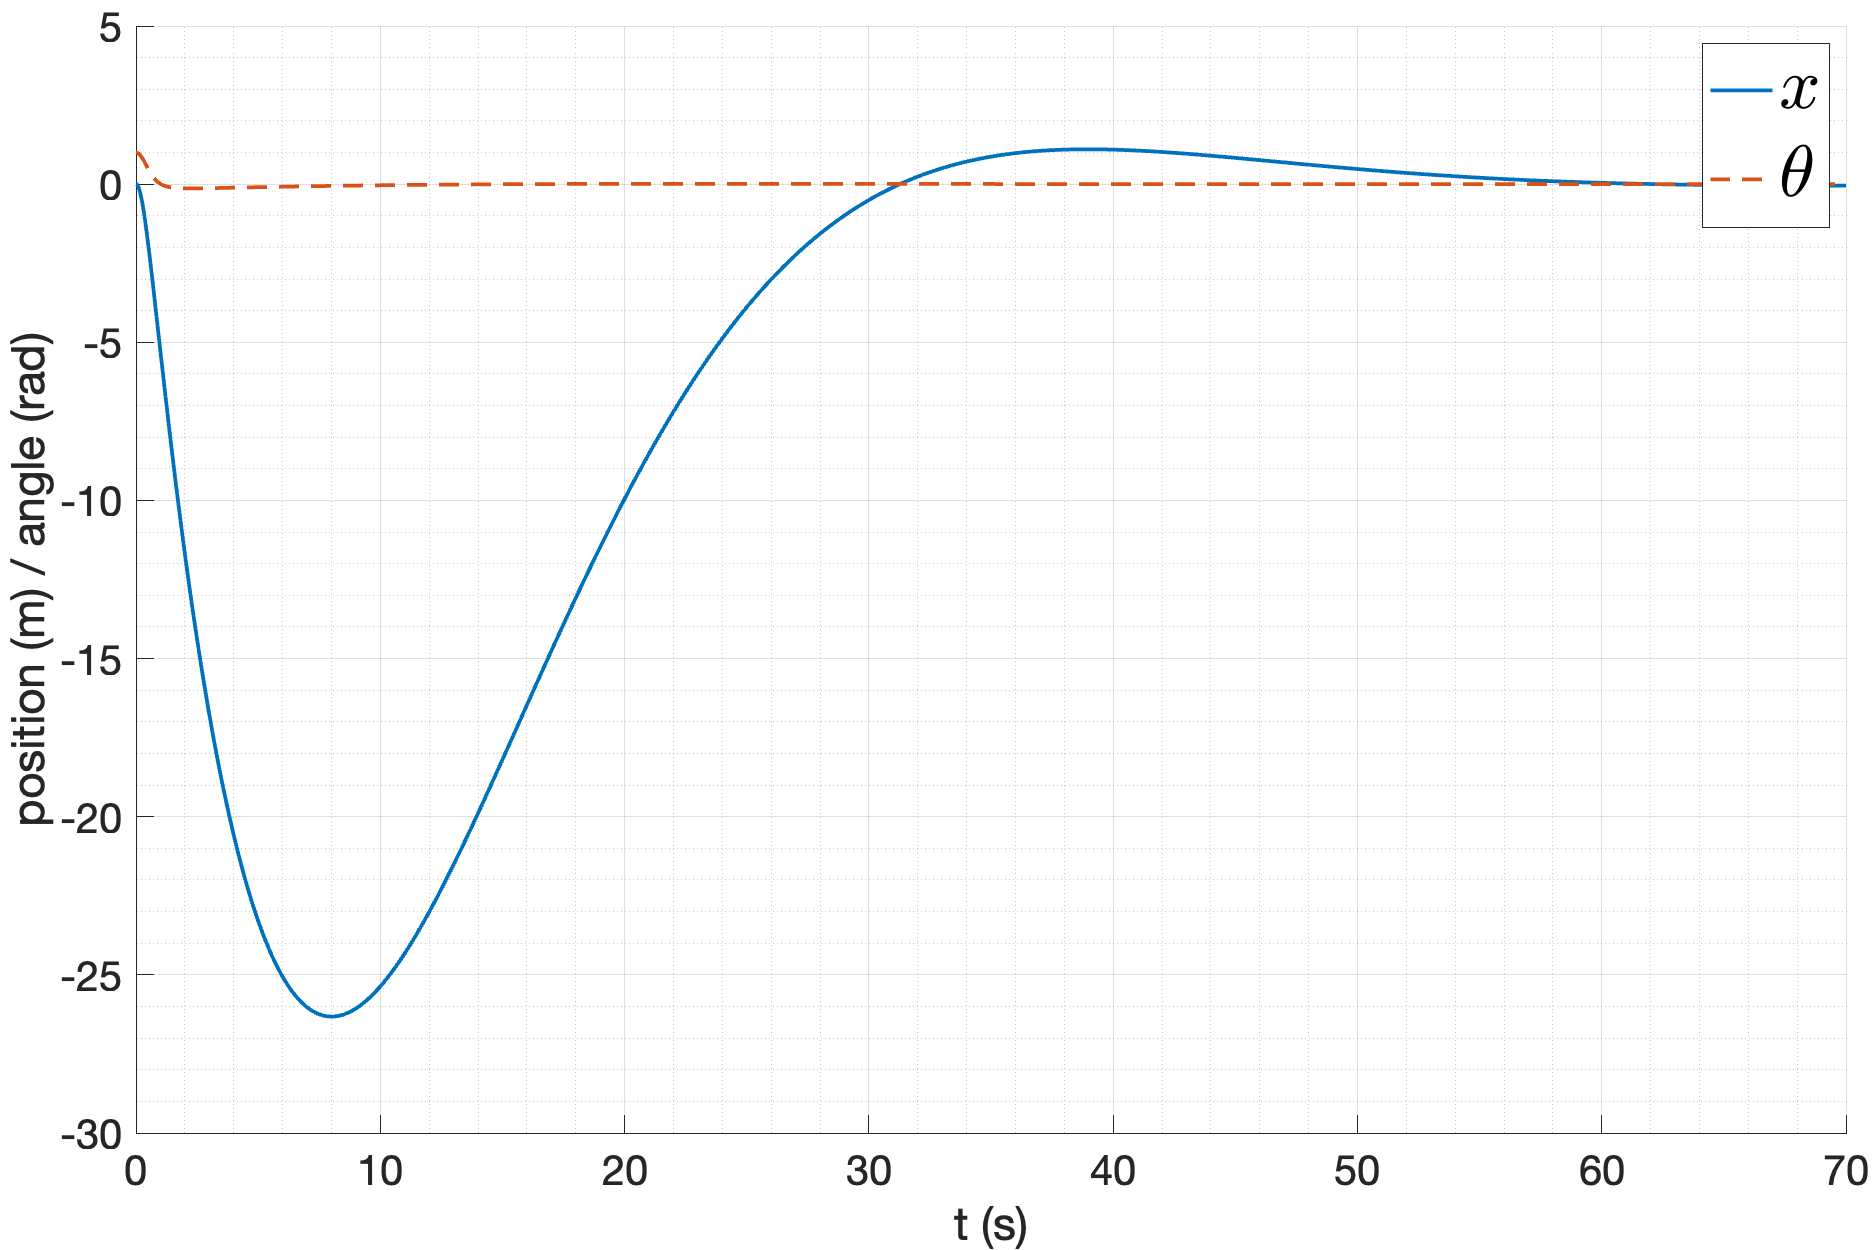
\includegraphics[width=\textwidth]{media/plots/LQR/out_3.png}
        \caption{Результат моделирования при $\theta_0 = 0.5$}
    \end{subfigure}
    \begin{subfigure}[b]{0.45\textwidth}
        \centering
        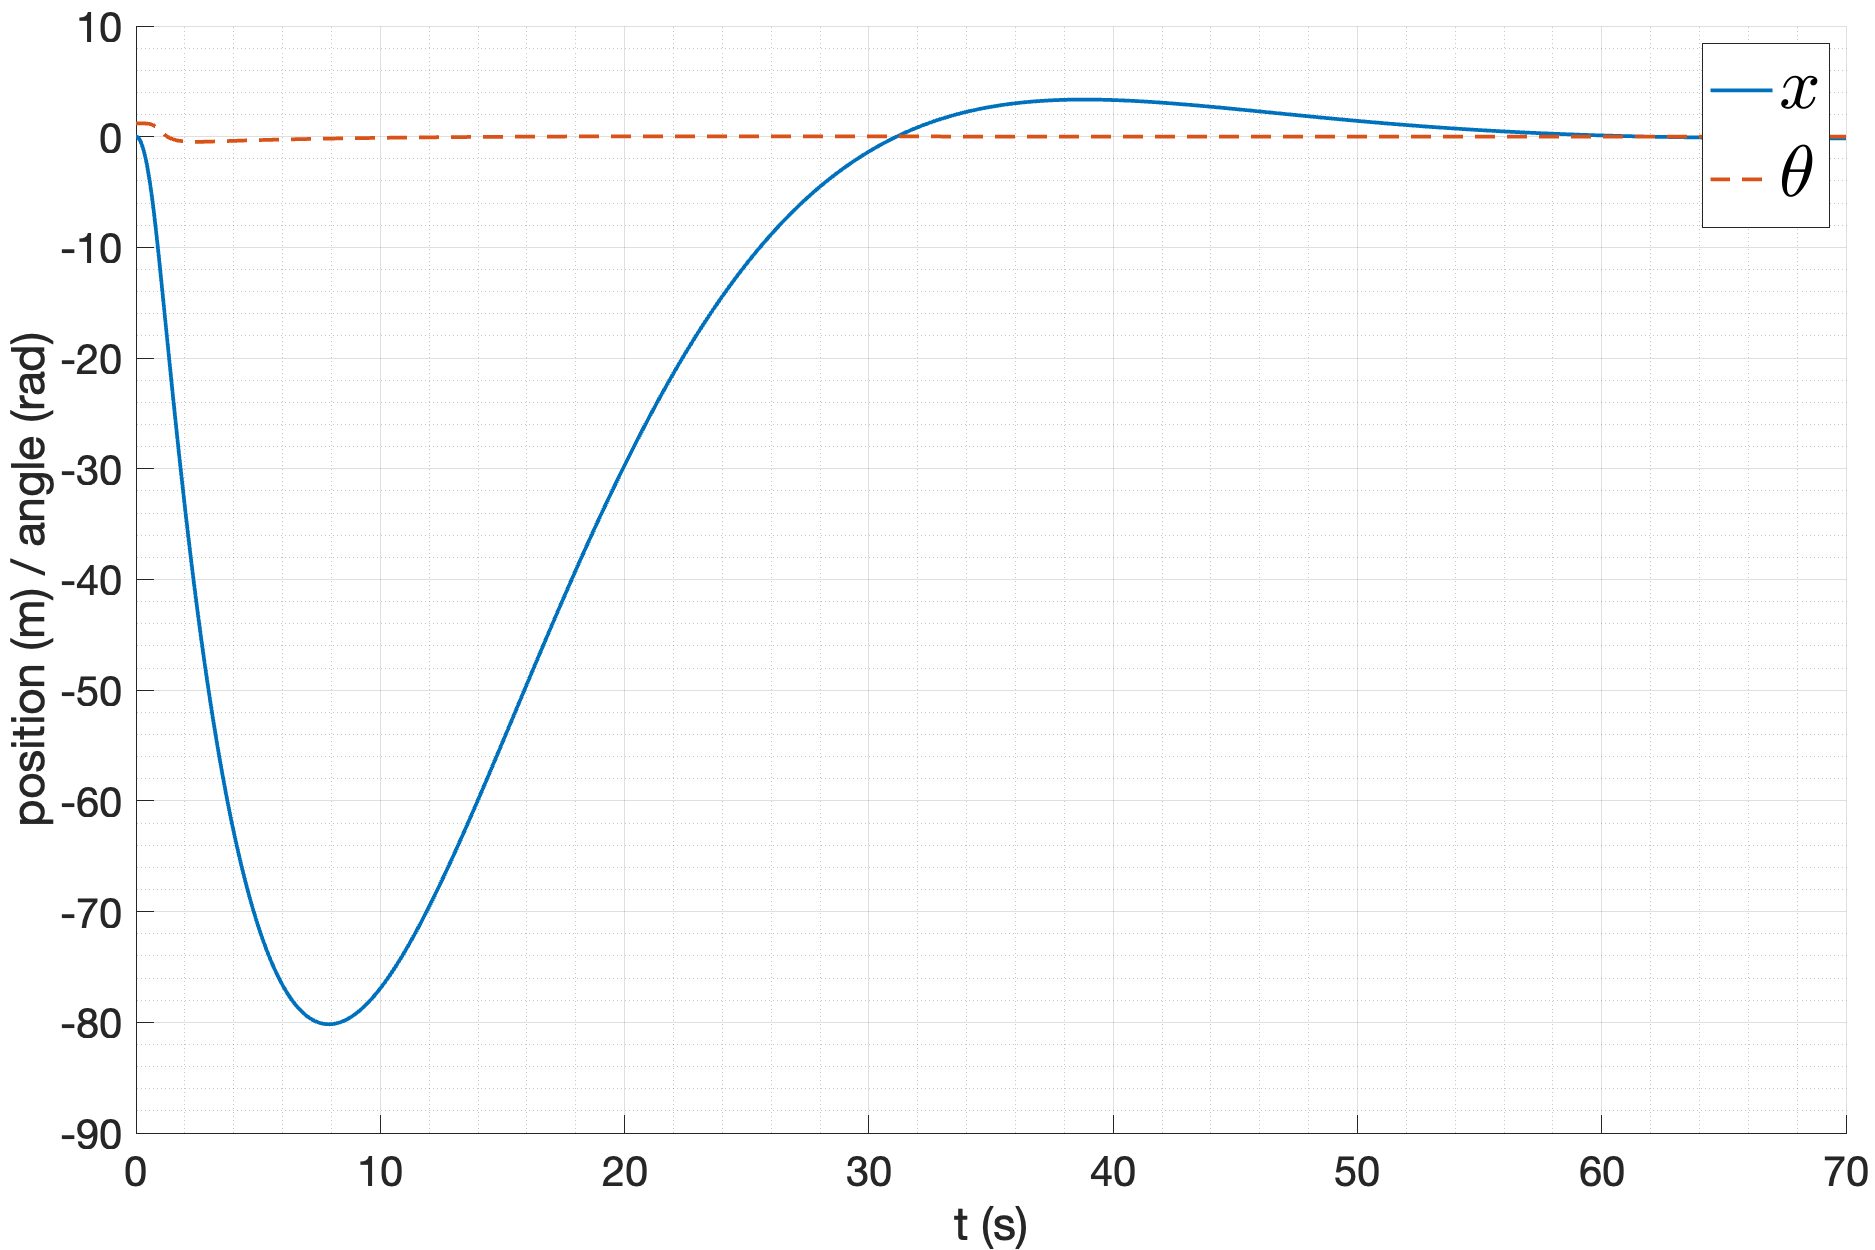
\includegraphics[width=\textwidth]{media/plots/LQR/out_4.png}
        \caption{Результат моделирования при $\theta_0 = 1.2$}
    \end{subfigure}
    \begin{subfigure}[b]{0.45\textwidth}
        \centering
        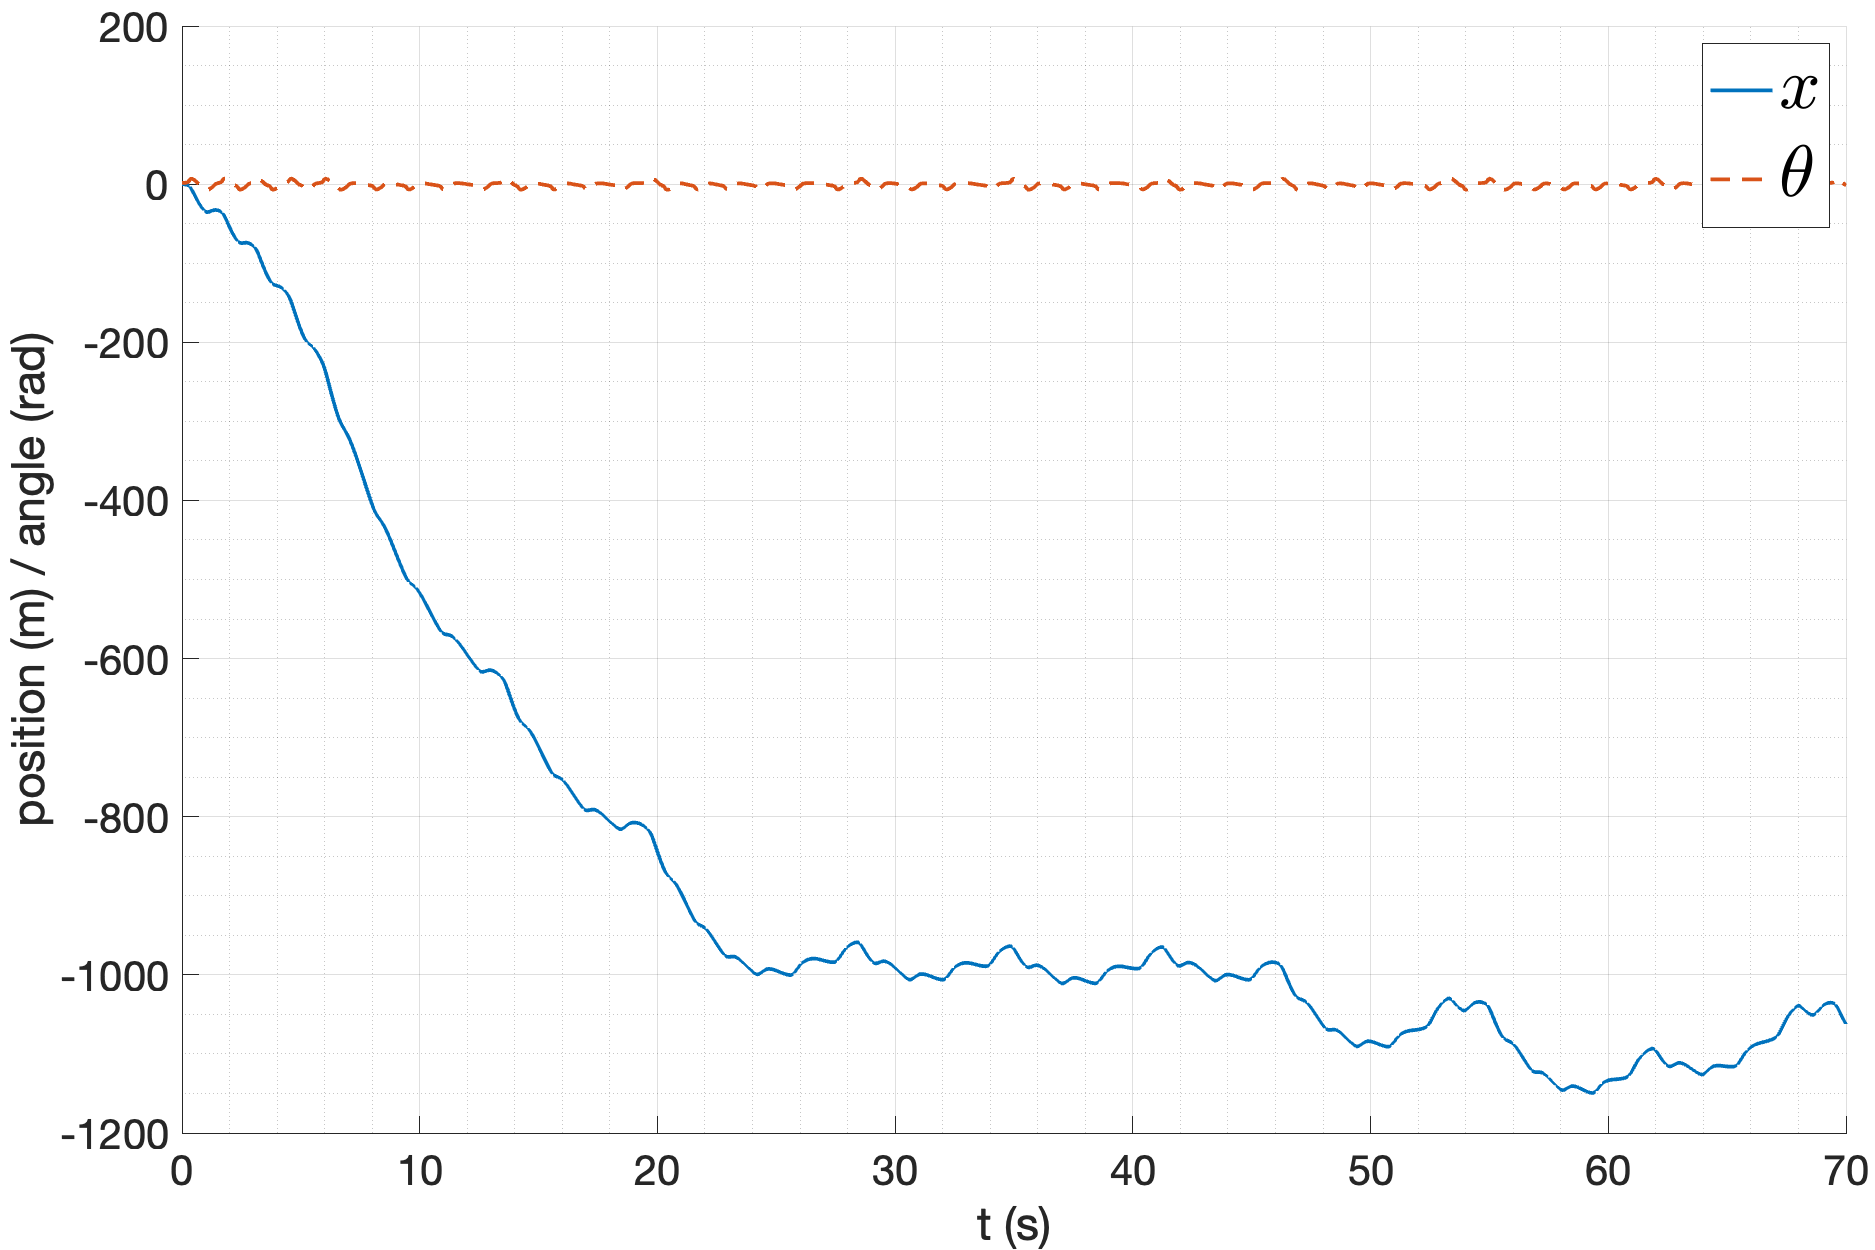
\includegraphics[width=\textwidth]{media/plots/LQR/out_5.png}
        \caption{Результат моделирования при $\theta_0 = 1.5$}
    \end{subfigure}
    \caption{Результат моделирования системы при различных начальных условиях}
    \label{fig:lqr_controller_2}
\end{figure}
Видно, что выход системы сходится к нулю при начальных отклонениях маятника вплоть до $1.2$ радиан.
При отклонении маятника в $1.5$ радиан система не может стабилизироваться, что, вероятнее всего, 
связано с тем, что отклонения реального поведения системы от ее линейной модели становятся значительными. 
    
Также можно заметить, что \textit{форма} переходного процесса остается практически неизменной при различных начальных условиях.
Это связано с тем, что синтез регулятора проводился по методу LQR, который обеспечивает оптимальное
управление в смысле минимизации функционала качества. 

\FloatBarrier
\subsection{Исследование переходного процесса}
Рассмотрим переходный процесс при различных весовых матрицах $Q$ и $R$. Матрица $R$ отвечает за 
штраф за \textit{агрессивное} управление, а матрица $Q$ отвечает за штраф за отклонение состояния системы от нуля.
Рассмотрим пары $(Q, R)$:
\begin{itemize}
    \item $Q = 30 \cdot I_{4\times 4}, R = 1$;
    \item $Q = 30 \cdot I_{4\times 4}, R = 10$;
    \item $Q = 200 \cdot I_{4\times 4}, R = 1$;
    \item $Q = 200 \cdot I_{4\times 4}, R = 10$;
\end{itemize}
Получаем следующие матрица регуляторов и значения функционала качества:
\begin{equation}
    \begin{array}{cccc}
        K_1 = \begin{bmatrix}
        5.48  & 56.48  & -5414.73  & -1223.92 \\ 
        \end{bmatrix} \\ 
        K_2 = \begin{bmatrix}
        1.73  & 31.04  & -5305.69  & -1198.97 \\ 
        \end{bmatrix} \\ 
        K_3 = \begin{bmatrix}
        10.00  & 77.80  & -5504.78  & -1244.53 \\
        \end{bmatrix} \\ 
        K_4 = \begin{bmatrix}
        3.16  & 42.37  & -5354.49  & -1210.13 \\ 
        \end{bmatrix} \\ 
    \end{array}
\end{equation}
Можно заметить, что компоненты, отвечающие за угол отклонения маятника и его угловую скорость значительно больше, 
чем компоненты, отвечающие за положение тележки и ее скорость. Это связано с тем, что маятник вносит большее 
влияние на устойчивость системы, так как является неустойчивым объектом. 

Переходные процесса для приведенных регуляторов представлены на рисунке \ref{fig:lqr_controller_qr}.
\begin{figure}[ht!]
    \centering
    \begin{subfigure}[b]{0.45\textwidth}
        \centering
        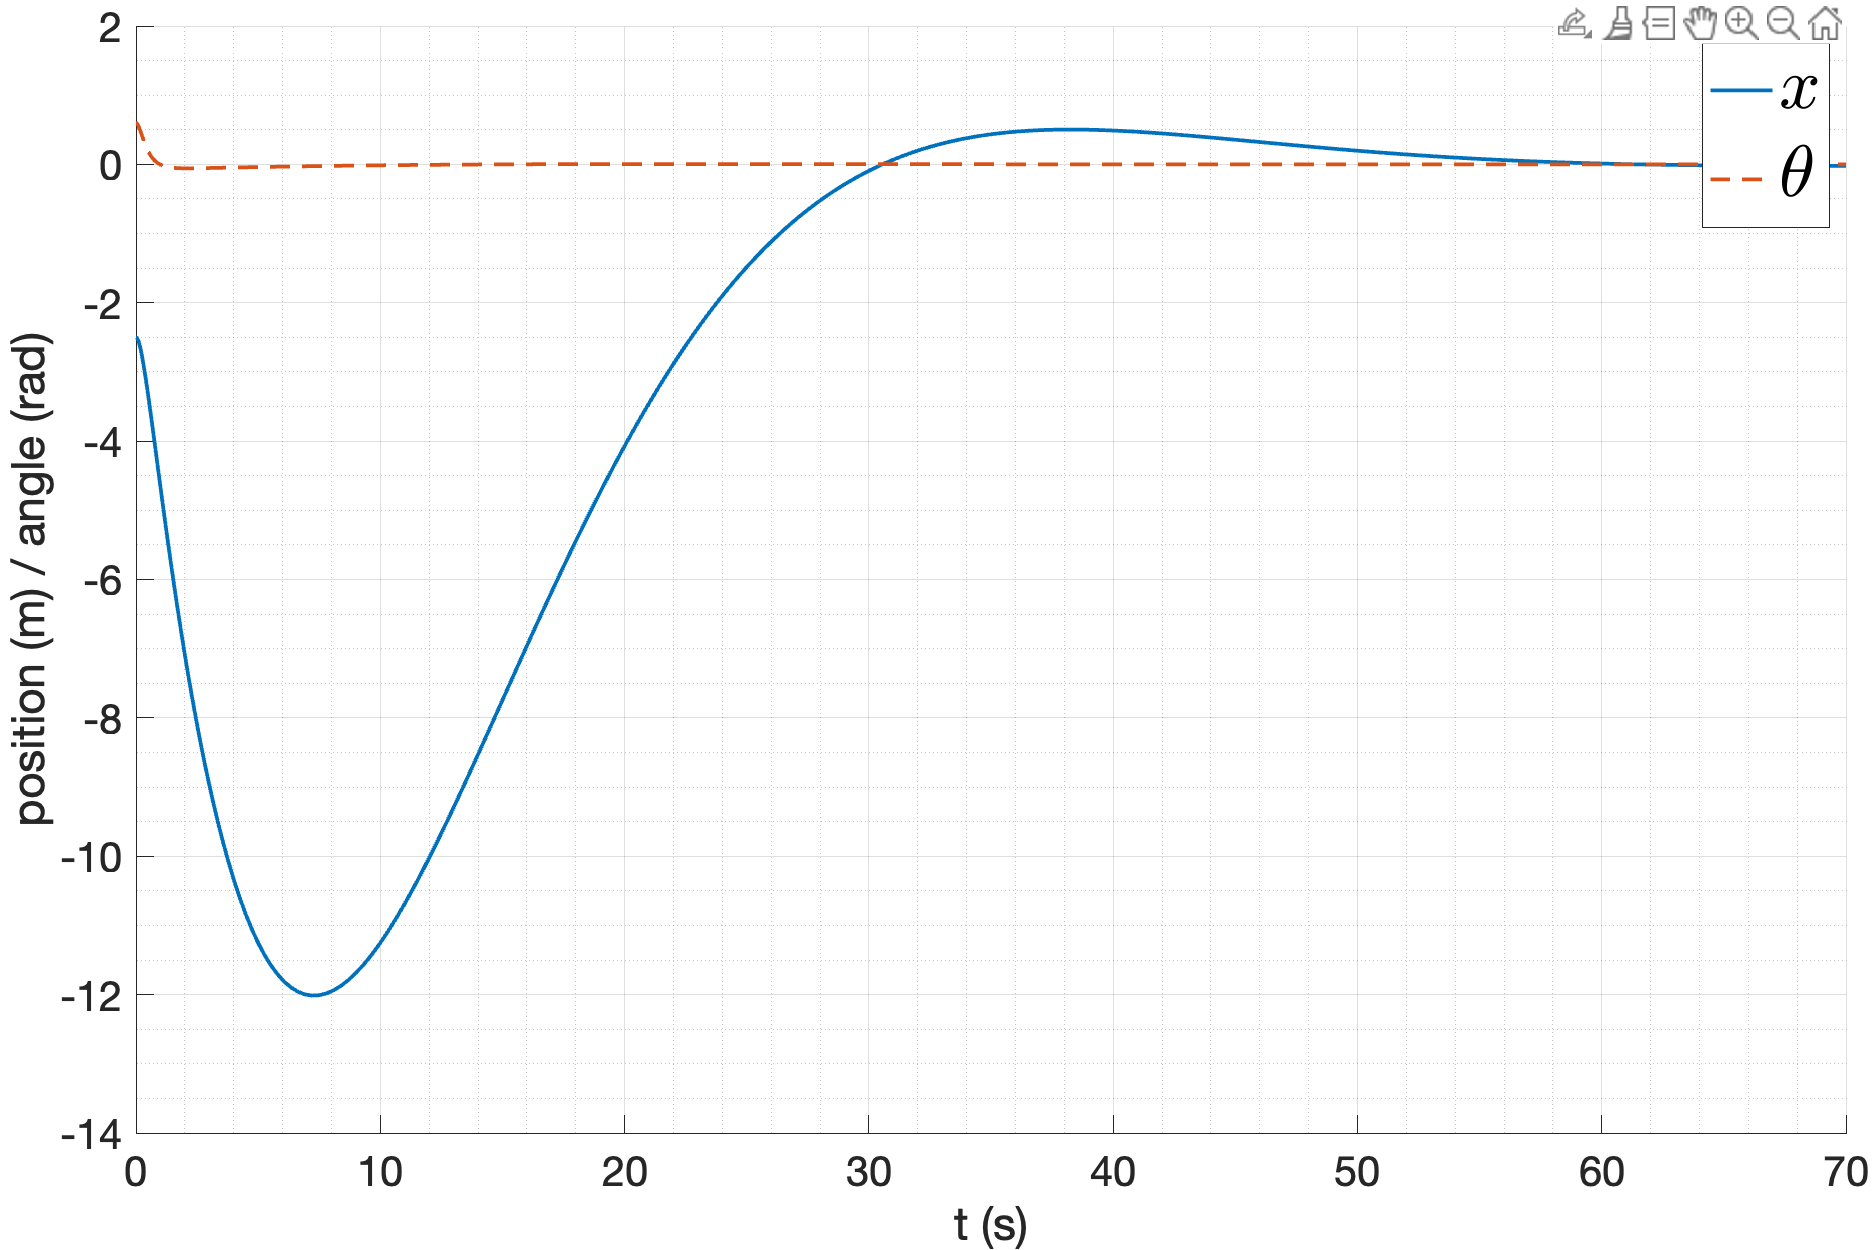
\includegraphics[width=\textwidth]{media/plots/LQR/out_6.png}
        \caption{Переходный процесс $Q = 30 \cdot I_{4\times 4}, R = 1$}
    \end{subfigure}
    \begin{subfigure}[b]{0.45\textwidth}
        \centering
        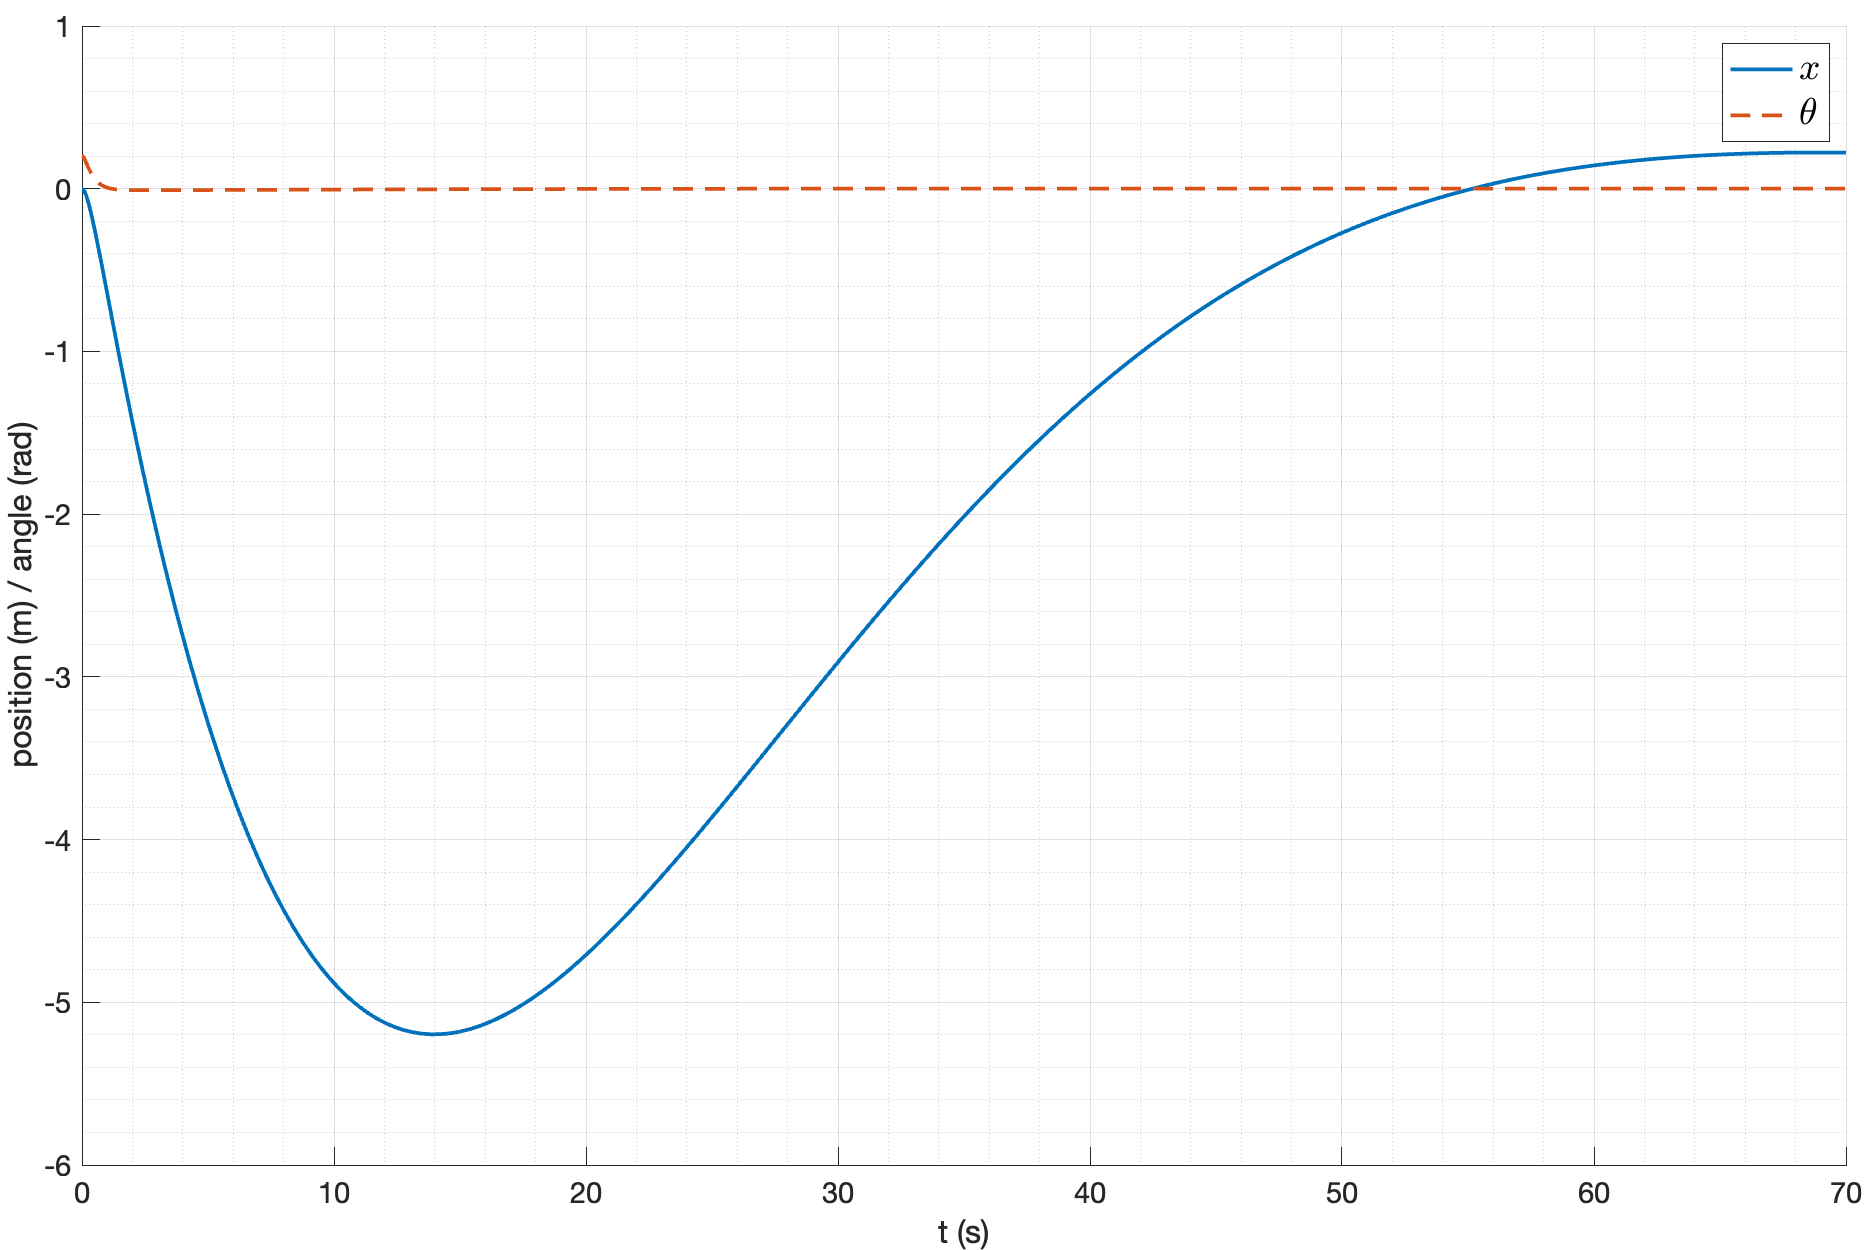
\includegraphics[width=\textwidth]{media/plots/LQR/out_7.png}
        \caption{Переходный процесс $Q = 30 \cdot I_{4\times 4}, R = 10$}
    \end{subfigure}
    \begin{subfigure}[b]{0.45\textwidth}
        \centering
        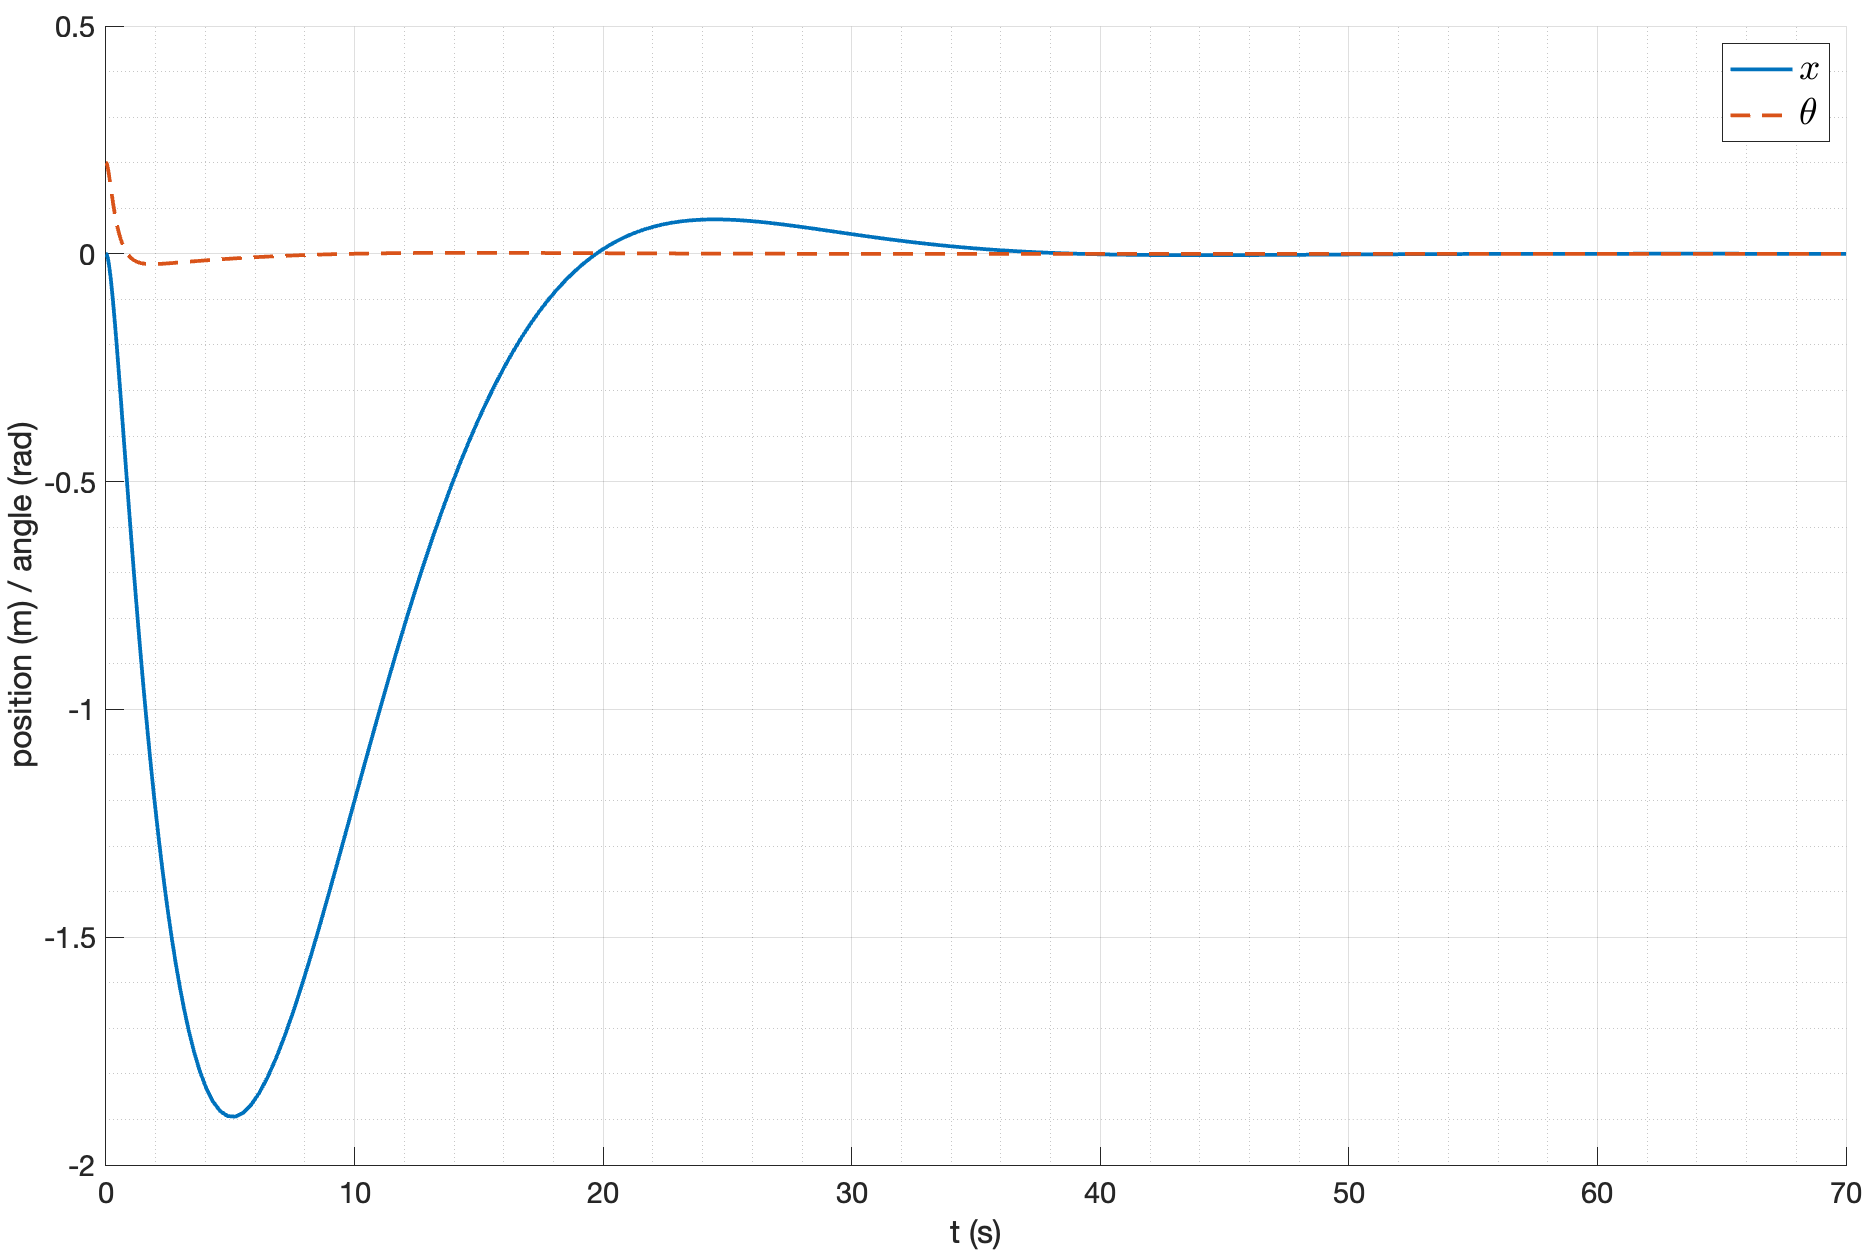
\includegraphics[width=\textwidth]{media/plots/LQR/out_8.png}
        \caption{Переходный процесс $Q = 200 \cdot I_{4\times 4}, R = 1$}
    \end{subfigure}
    \begin{subfigure}[b]{0.45\textwidth}
        \centering
        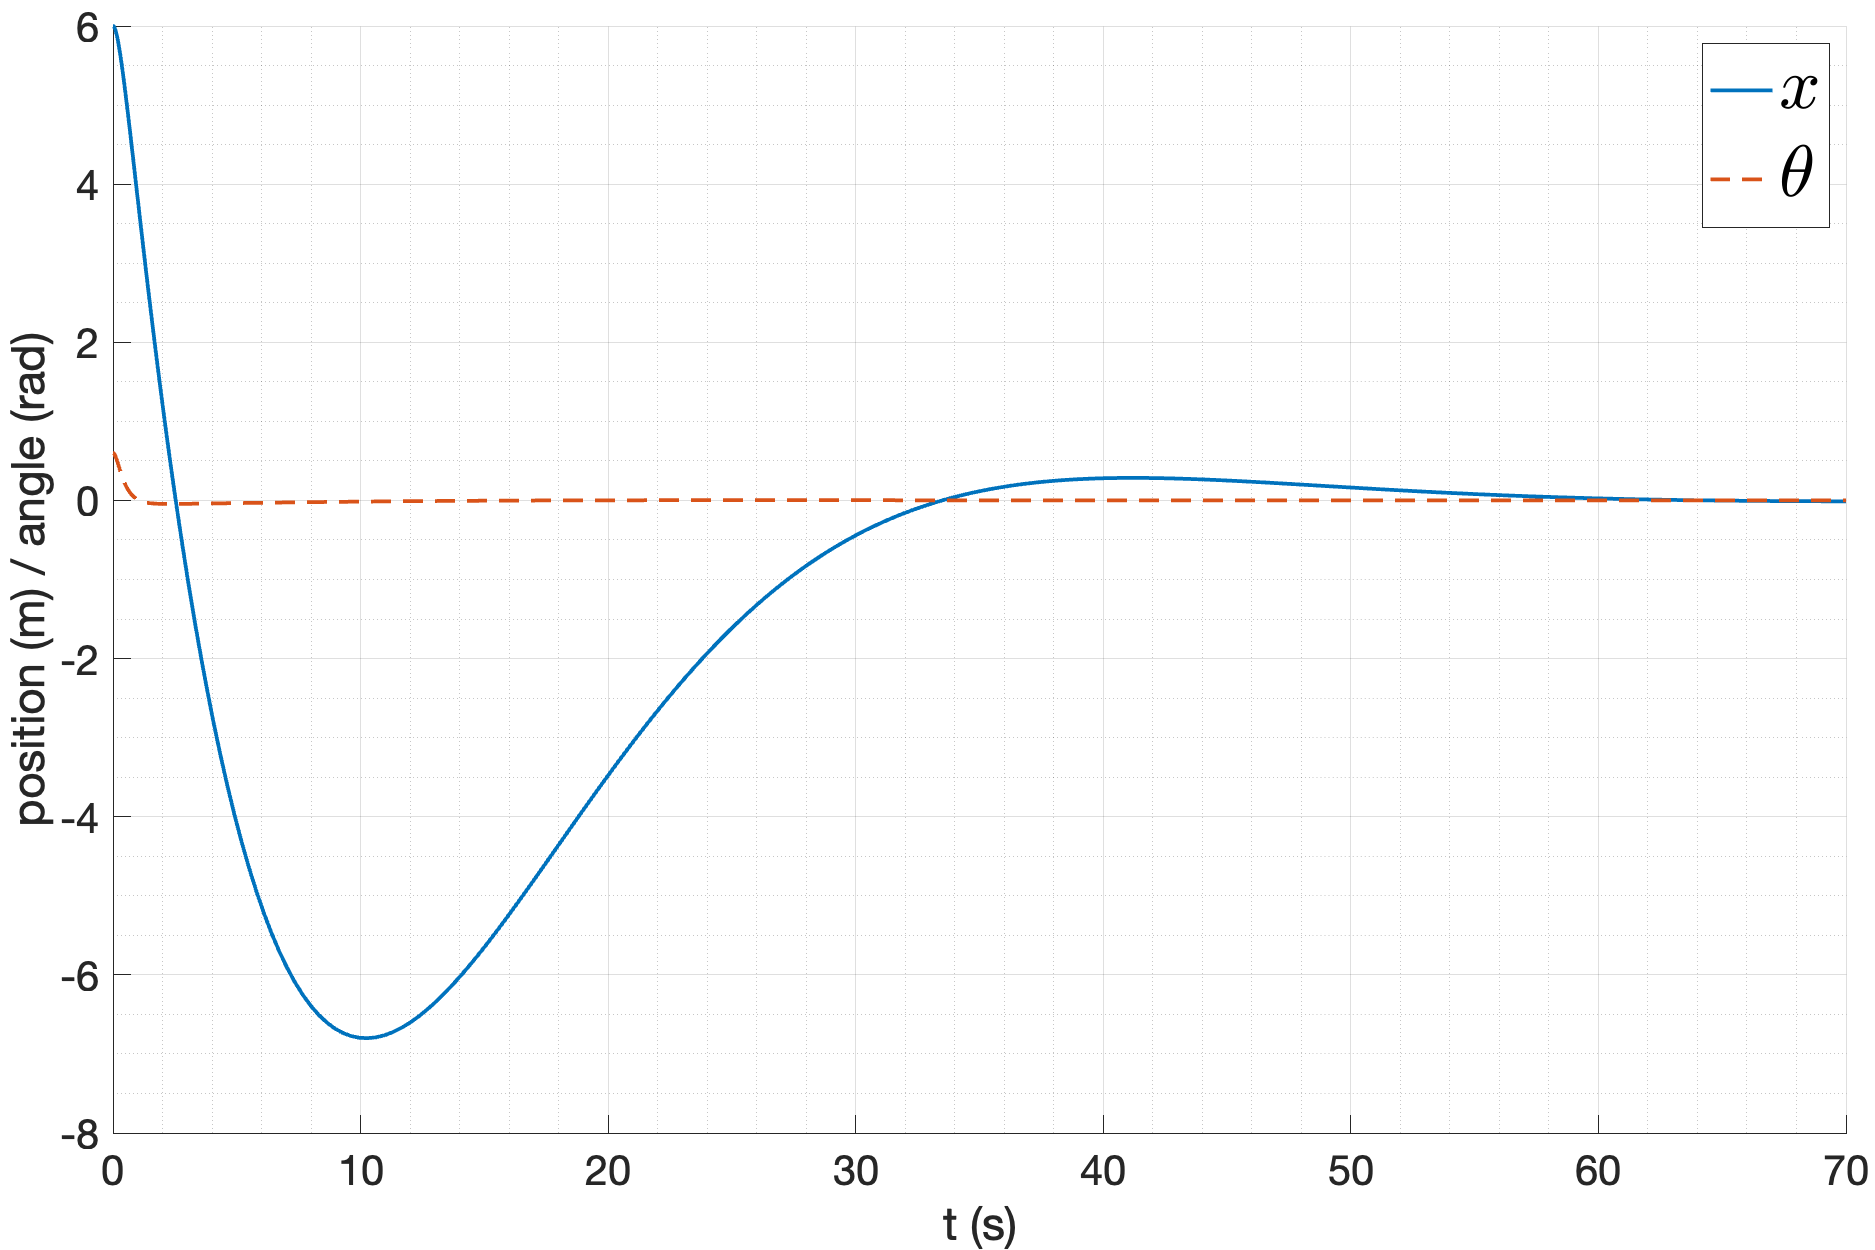
\includegraphics[width=\textwidth]{media/plots/LQR/out_9.png}
        \caption{Переходный процесс $Q = 200 \cdot I_{4\times 4}, R = 10$}
    \end{subfigure}
    \caption{Переходные процессы для различных весовых матриц $Q$ и $R$}
    \label{fig:lqr_controller_qr}
\end{figure} 
Видно, что при увеличении матрицы $Q$ переходный процесс становится более быстрым, матрица $Q$ отвечает 
за штраф за отклонение состояния системы от нуля, поэтому при увеличении ее значений системы меньше 
отклоняется от состояния равновесия. При увеличении матрицы $R$ переходный процесс становится более медленным,
так как матрица $R$ отвечает за штраф за \textit{агрессивное} управление, поэтому при увеличении ее значений 
мы получаем более плавное управление, что приводит к более медленному переходному процессу. 

\FloatBarrier
\subsection{Фильтр Калмана}
Синтезируем фильтр Калмана с матрицами
\begin{equation}
    Q = 30 \cdot \cdot I_{4\times 4}, \quad R = 1
\end{equation}
решая уравнение Риккати при $v = 1$:
\begin{equation}
    \begin{cases}
        A^T + PA^T + Q - vPCR^{-1}B^CP = 0 \\ 
        L = -PC^TR^{-1}
    \end{cases}
\end{equation}
Условием существования решения является обнаруживаемость пары $(A, C)$ и управляемость пары $(A, Q)$. 
Получаем матрицу фильтра Калмана
\begin{equation}
    L = \begin{bmatrix}
        -6.40  & -0.04 \\ 
        -5.48  & -0.41 \\ 
        -0.04  & -10.48 \\ 
        -0.20  & -39.94 \\ 
    \end{bmatrix}
\end{equation}
Проверим работу полученного фильтра Калмана, проведя моделирование замкнутой системы, рассмотренной ранее 
с нулевыми начальными условиями для фильтра Калмана. Результат моделирования представлен на рисунке \ref{fig:kalman_filter} и 
\ref{fig:kalman_filter_err}
\begin{figure}[ht!]
    \centering
    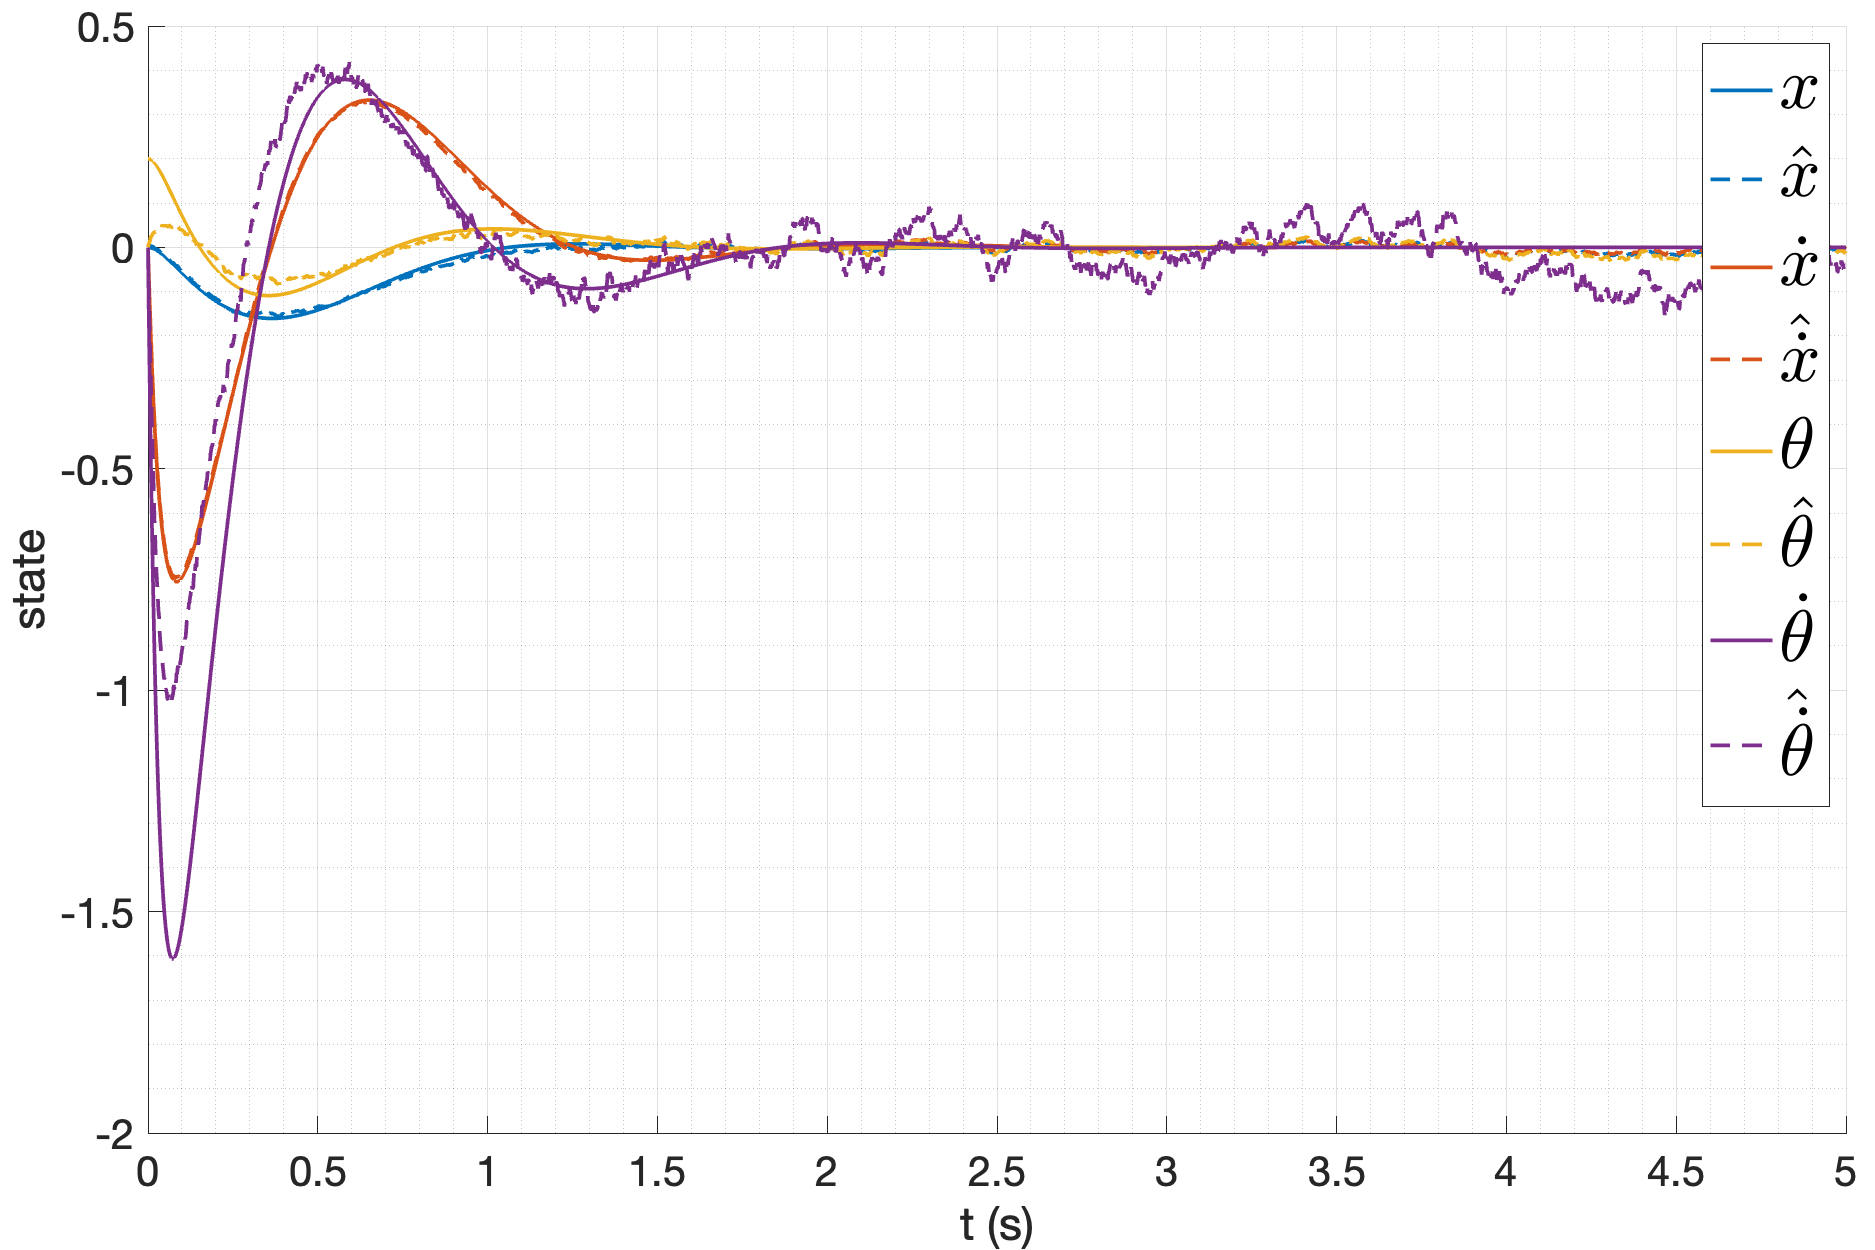
\includegraphics[width=\textwidth]{media/plots/kalman/observer_cmp_1.png}
    \caption{Реальное состояние системы и оценка состояния фильтром Калмана}
    \label{fig:kalman_filter}
\end{figure}
\begin{figure}[ht!]
    \centering
    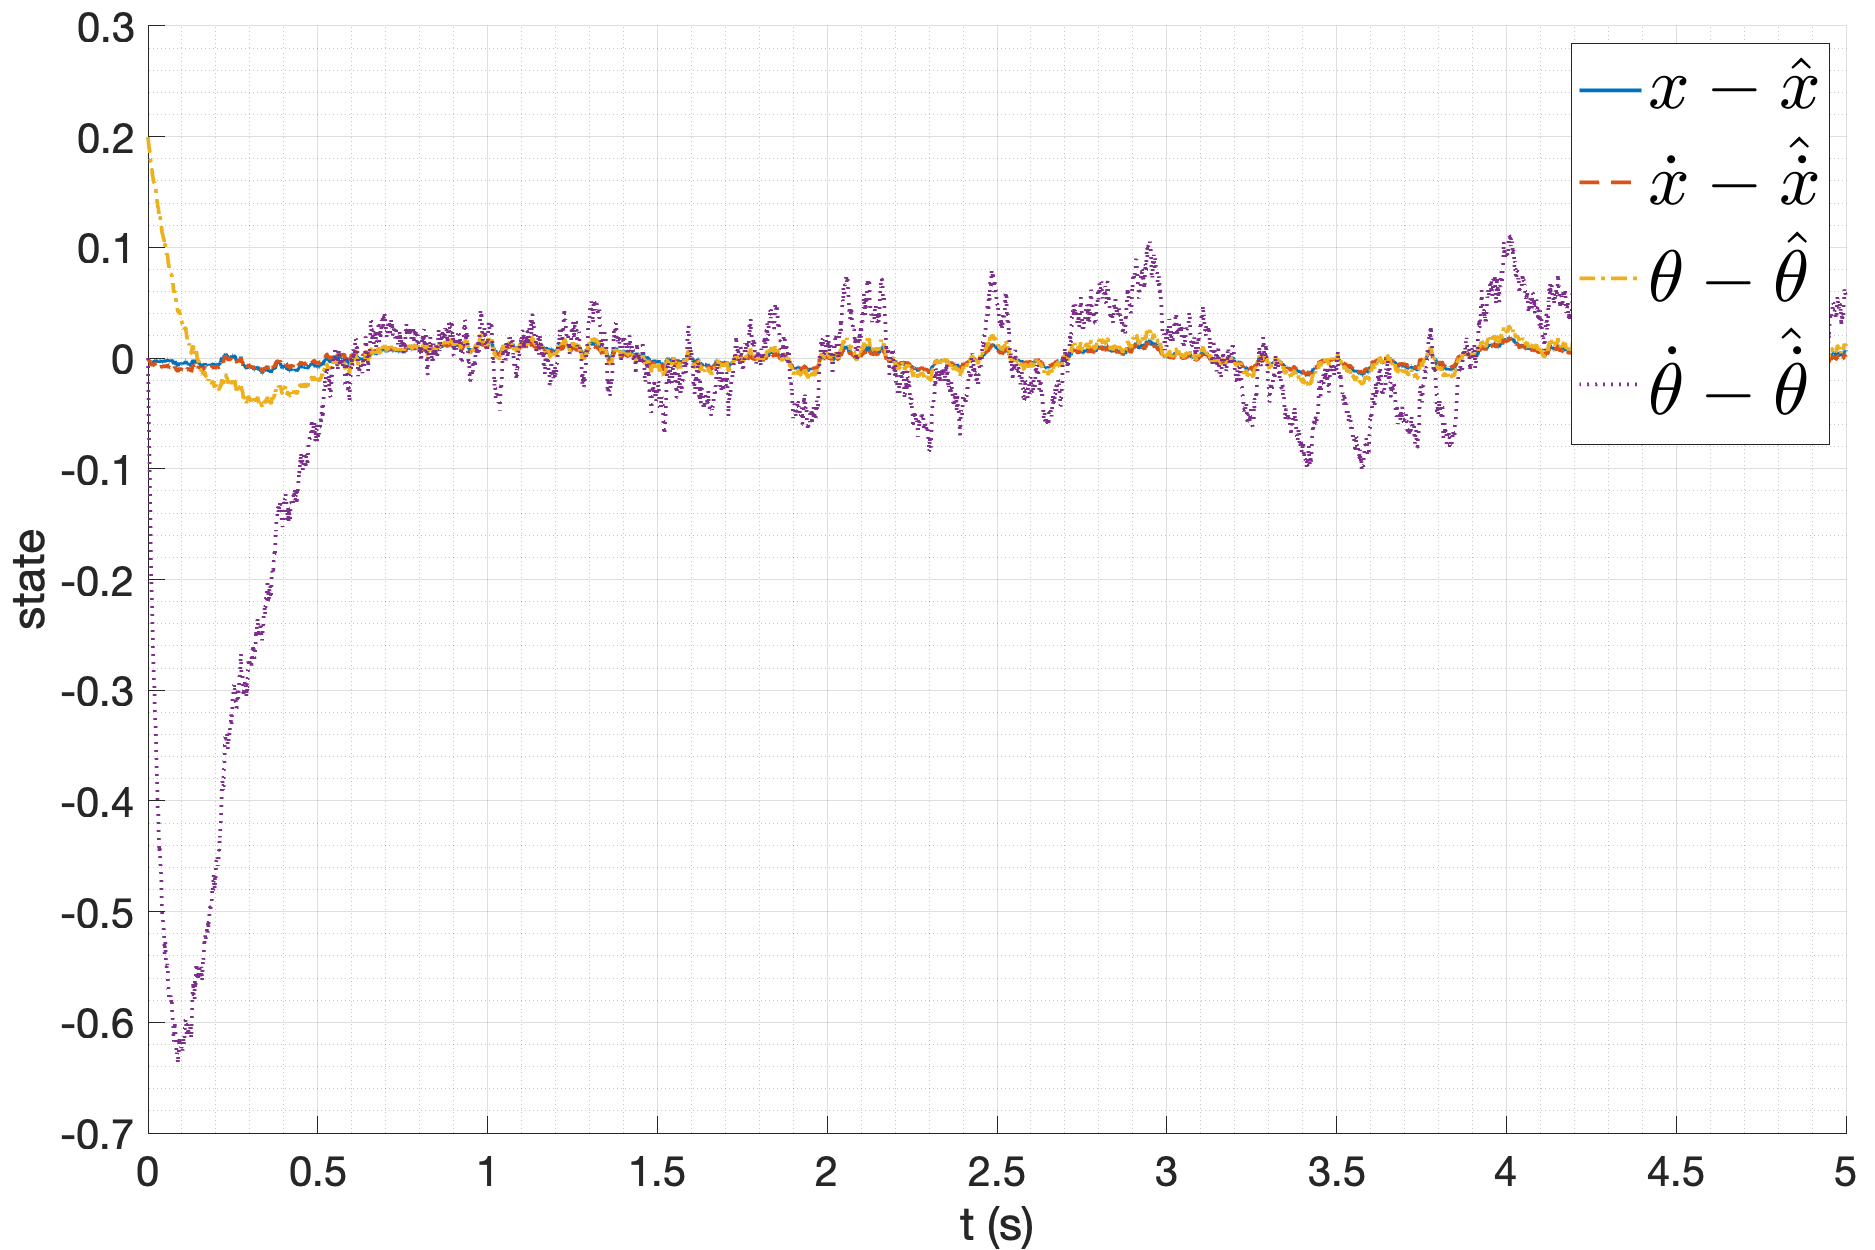
\includegraphics[width=\textwidth]{media/plots/kalman/observer_err_1.png}
    \caption{Оценка ошибки фильтра Калмана}
    \label{fig:kalman_filter_err}
\end{figure}
Видно, при оценка состояние системы фильтром Калмана достаточно близка к реальному состоянию системы. При этом 
можно заметить более быструю сходимость компонент, связанных с тележкой, что может быть обусловлено тем, что 
начально положение тележки было нулевым, как и начальное состояние фильтра Калмана. 

\FloatBarrier
\subsection{LQG для линейной модели}
Будем использовать LQR регулятор совместно с фильтром Калмана для управления линейной моделью системы в 
условиях, когда состояние системы не может быть измерено напрямую, при этом в измеряемых компонентах присутствует 
белый шум. 

Будем рассматривать систему c внешним возмущением и шумом: 
\begin{equation}
    \begin{cases}
        \dot{x} = Ax + Bu + Df \\ 
        y = Cx + \epsilon
    \end{cases}
\end{equation}
где $f$ и $\epsilon$ --- белый шум c дисперсиями $var_f = 0.5$ и $var_\epsilon = 0.1$ соответственно.

Используя то, что дисперсии белого шуми известны, можно синтезировать фильтр Калмана, с матрицами 
\begin{equation}
    Q = var_f \cdot I_{4\times 4}, \quad R = var_\epsilon
\end{equation}
Решив уравнение Риккати при $v = 1$, получаем матрицу фильтра Калмана: 
\begin{equation}
    L = \begin{bmatrix}
        -3.08  & -0.06 \\ 
        -2.24  & -0.44 \\ 
        -0.06  & -9.14 \\ 
        -0.28  & -39.31 \\ 
    \end{bmatrix}
\end{equation}
Проверим работу полученного фильтра Калмана, проведя моделирование. Результаты моделирования представлены на рисунке \ref{fig:lqg_filter}. 
\begin{figure}[ht!]
    \centering
    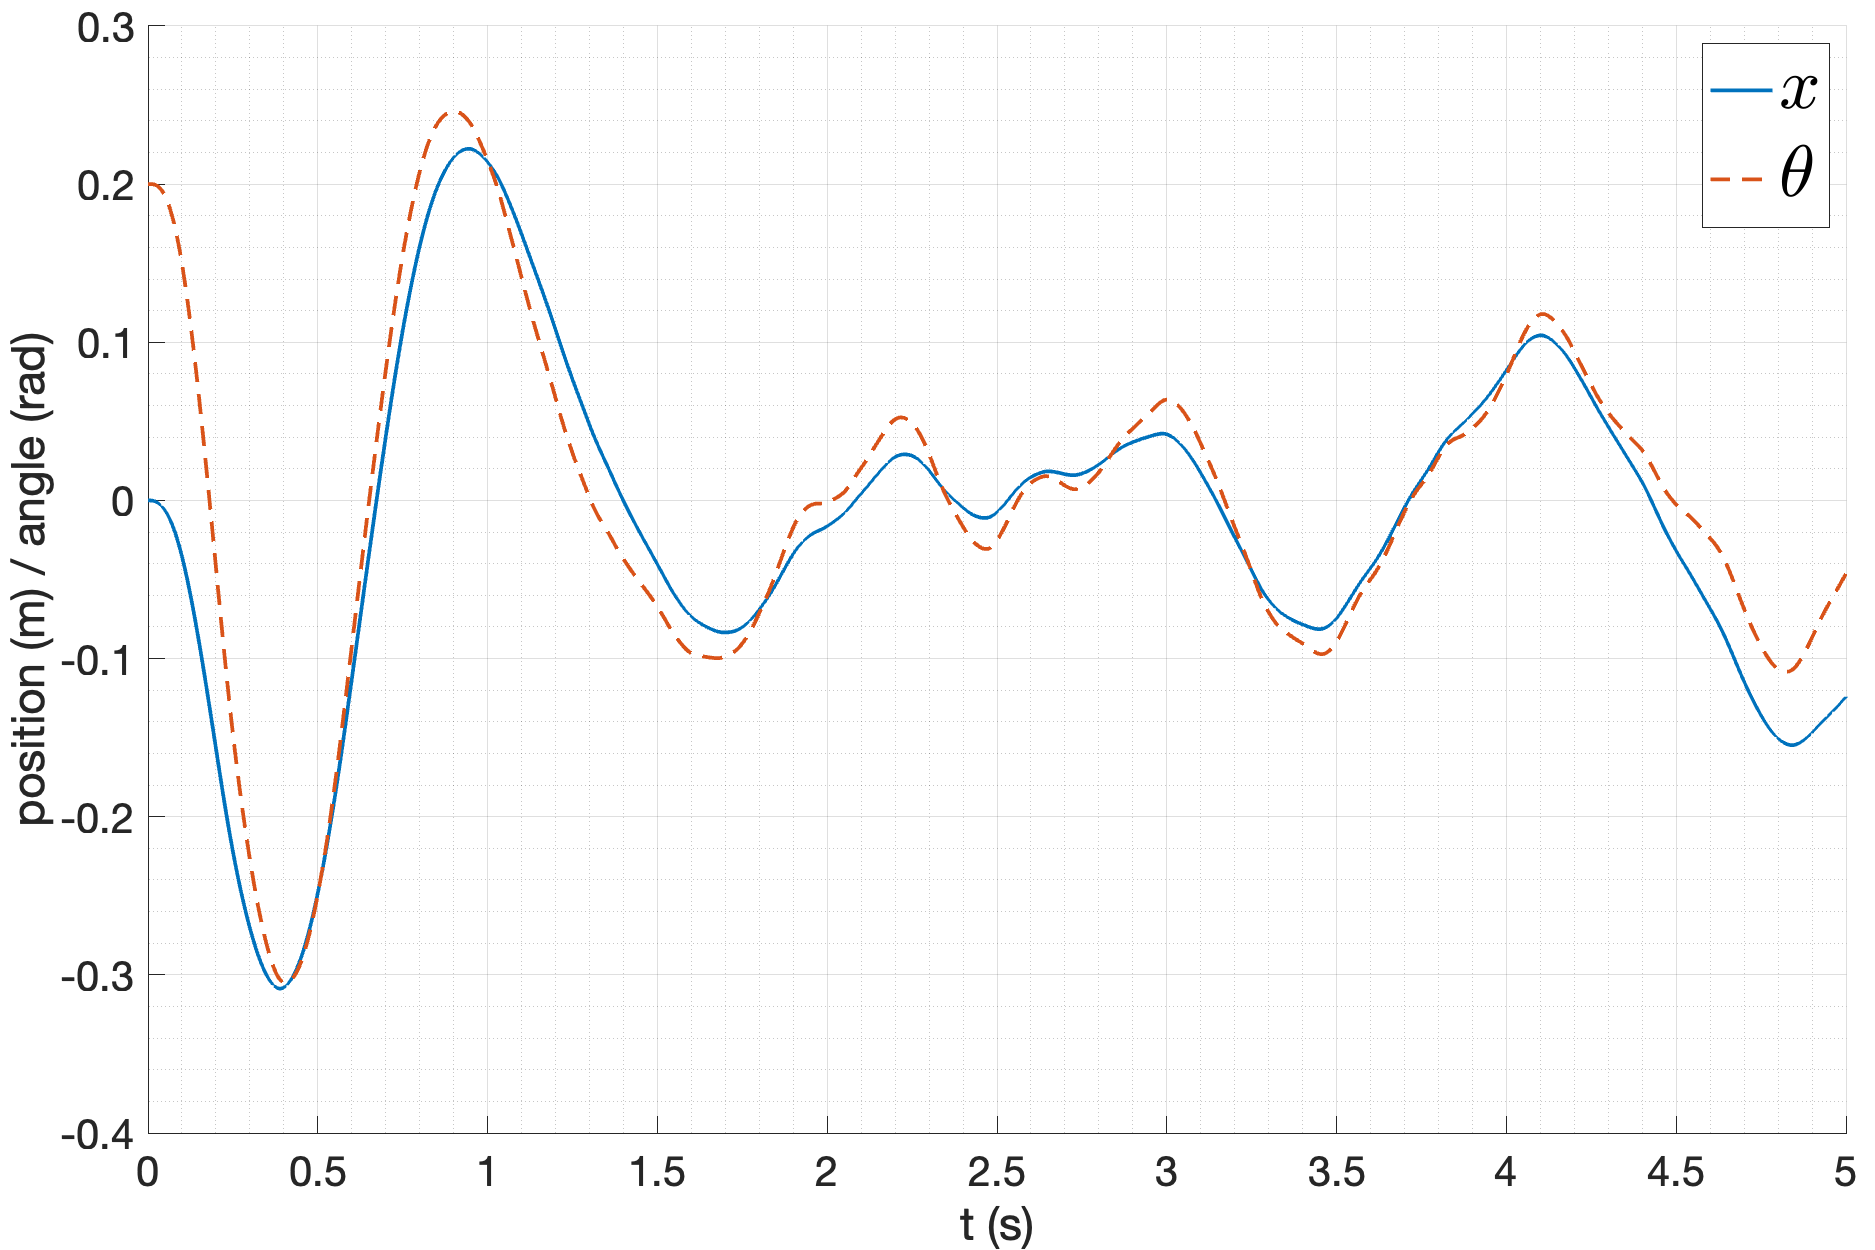
\includegraphics[width=\textwidth]{media/plots/LQG/out_1.png}
    \caption{Выход системы при использовании LQG регулятора}
    \label{fig:lqg_filter}
\end{figure}
Вход регулятора (зашумленный выход системы) представлен на рисунке \ref{fig:lqg_filter_y}. 
\begin{figure}[ht!]
    \begin{subfigure}[b]{0.45\textwidth}
        \centering
        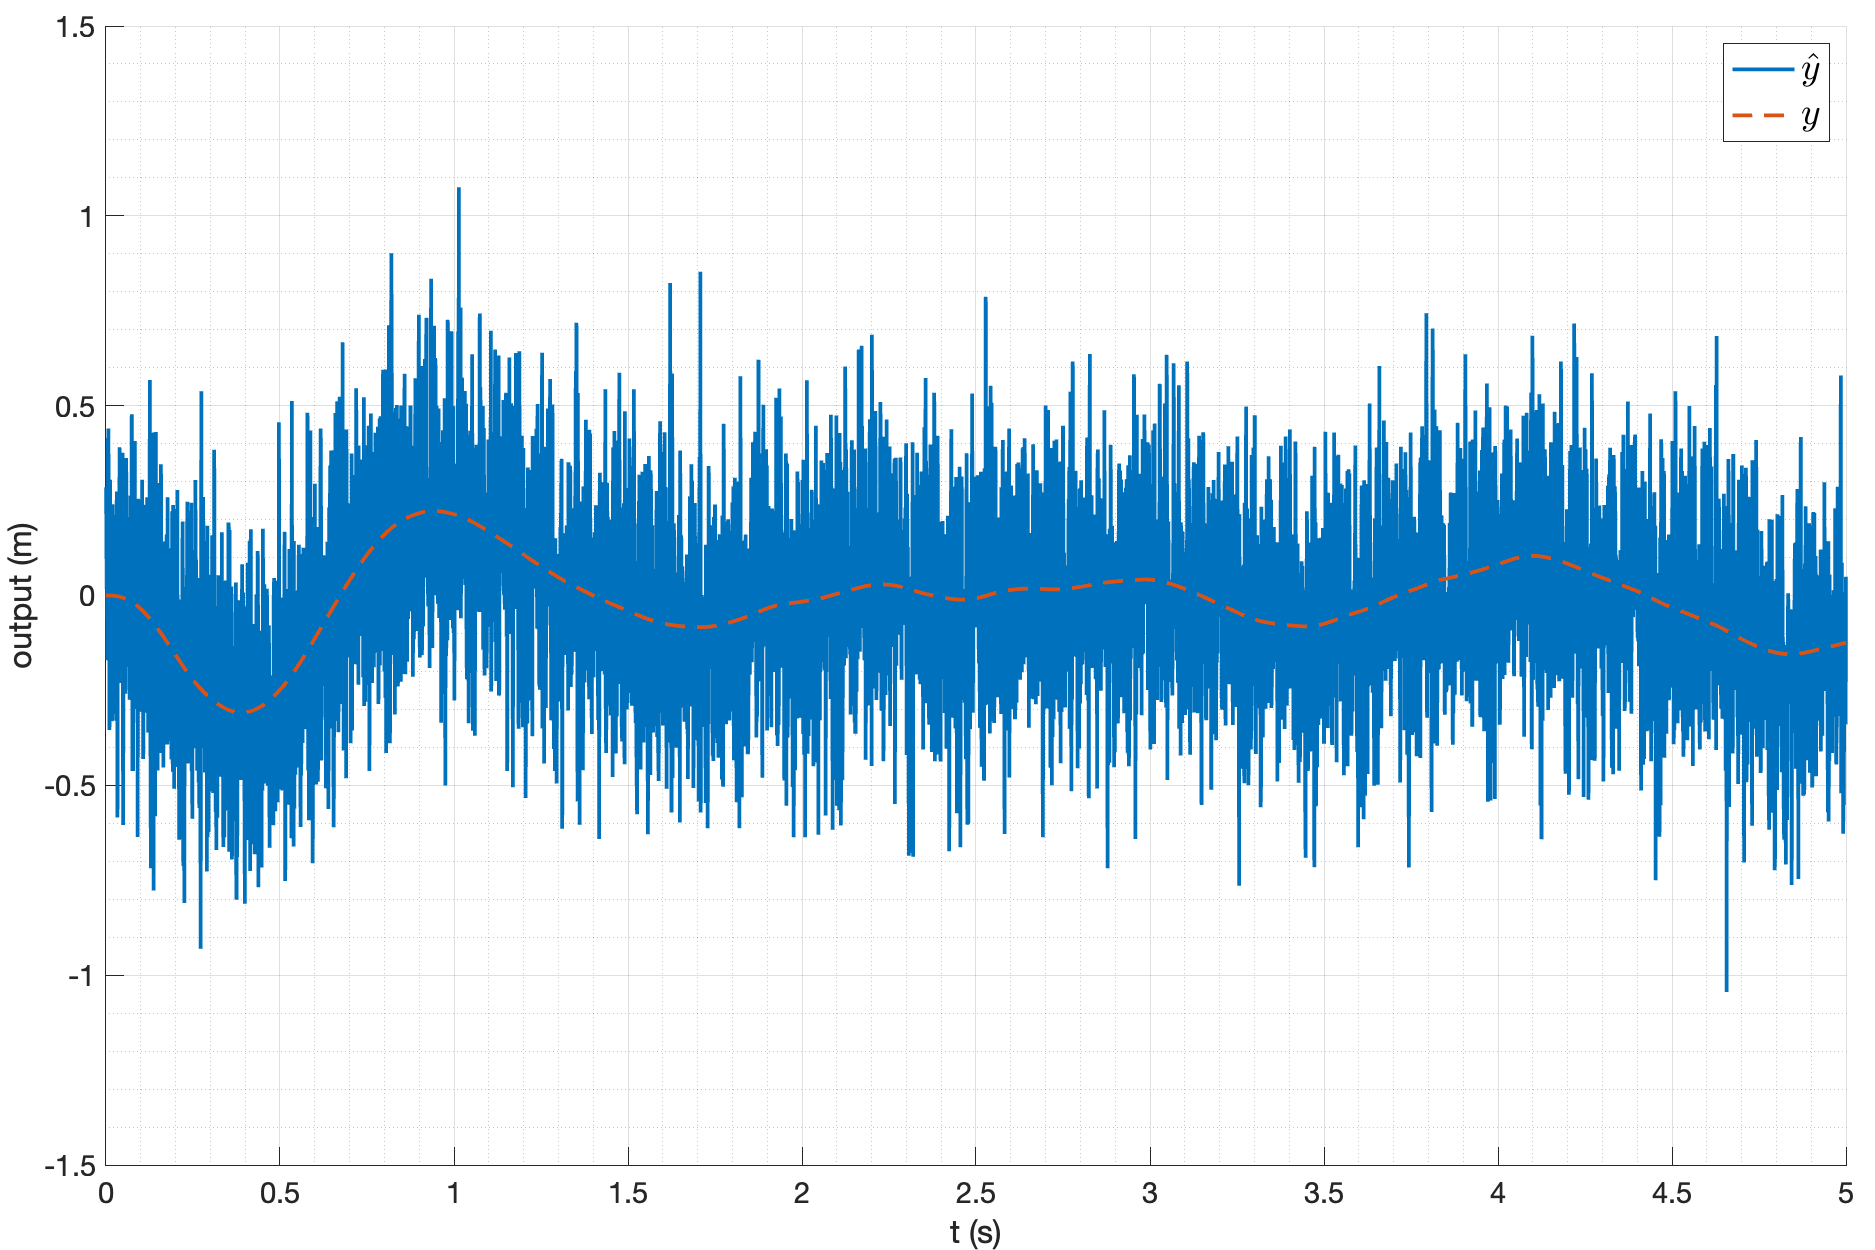
\includegraphics[width=\textwidth]{media/plots/LQG/observer_y1_cmp_1.png}
        \caption{Выход системы с шумом (компонента $y_1$)}
    \end{subfigure}
    \begin{subfigure}[b]{0.45\textwidth}
        \centering
        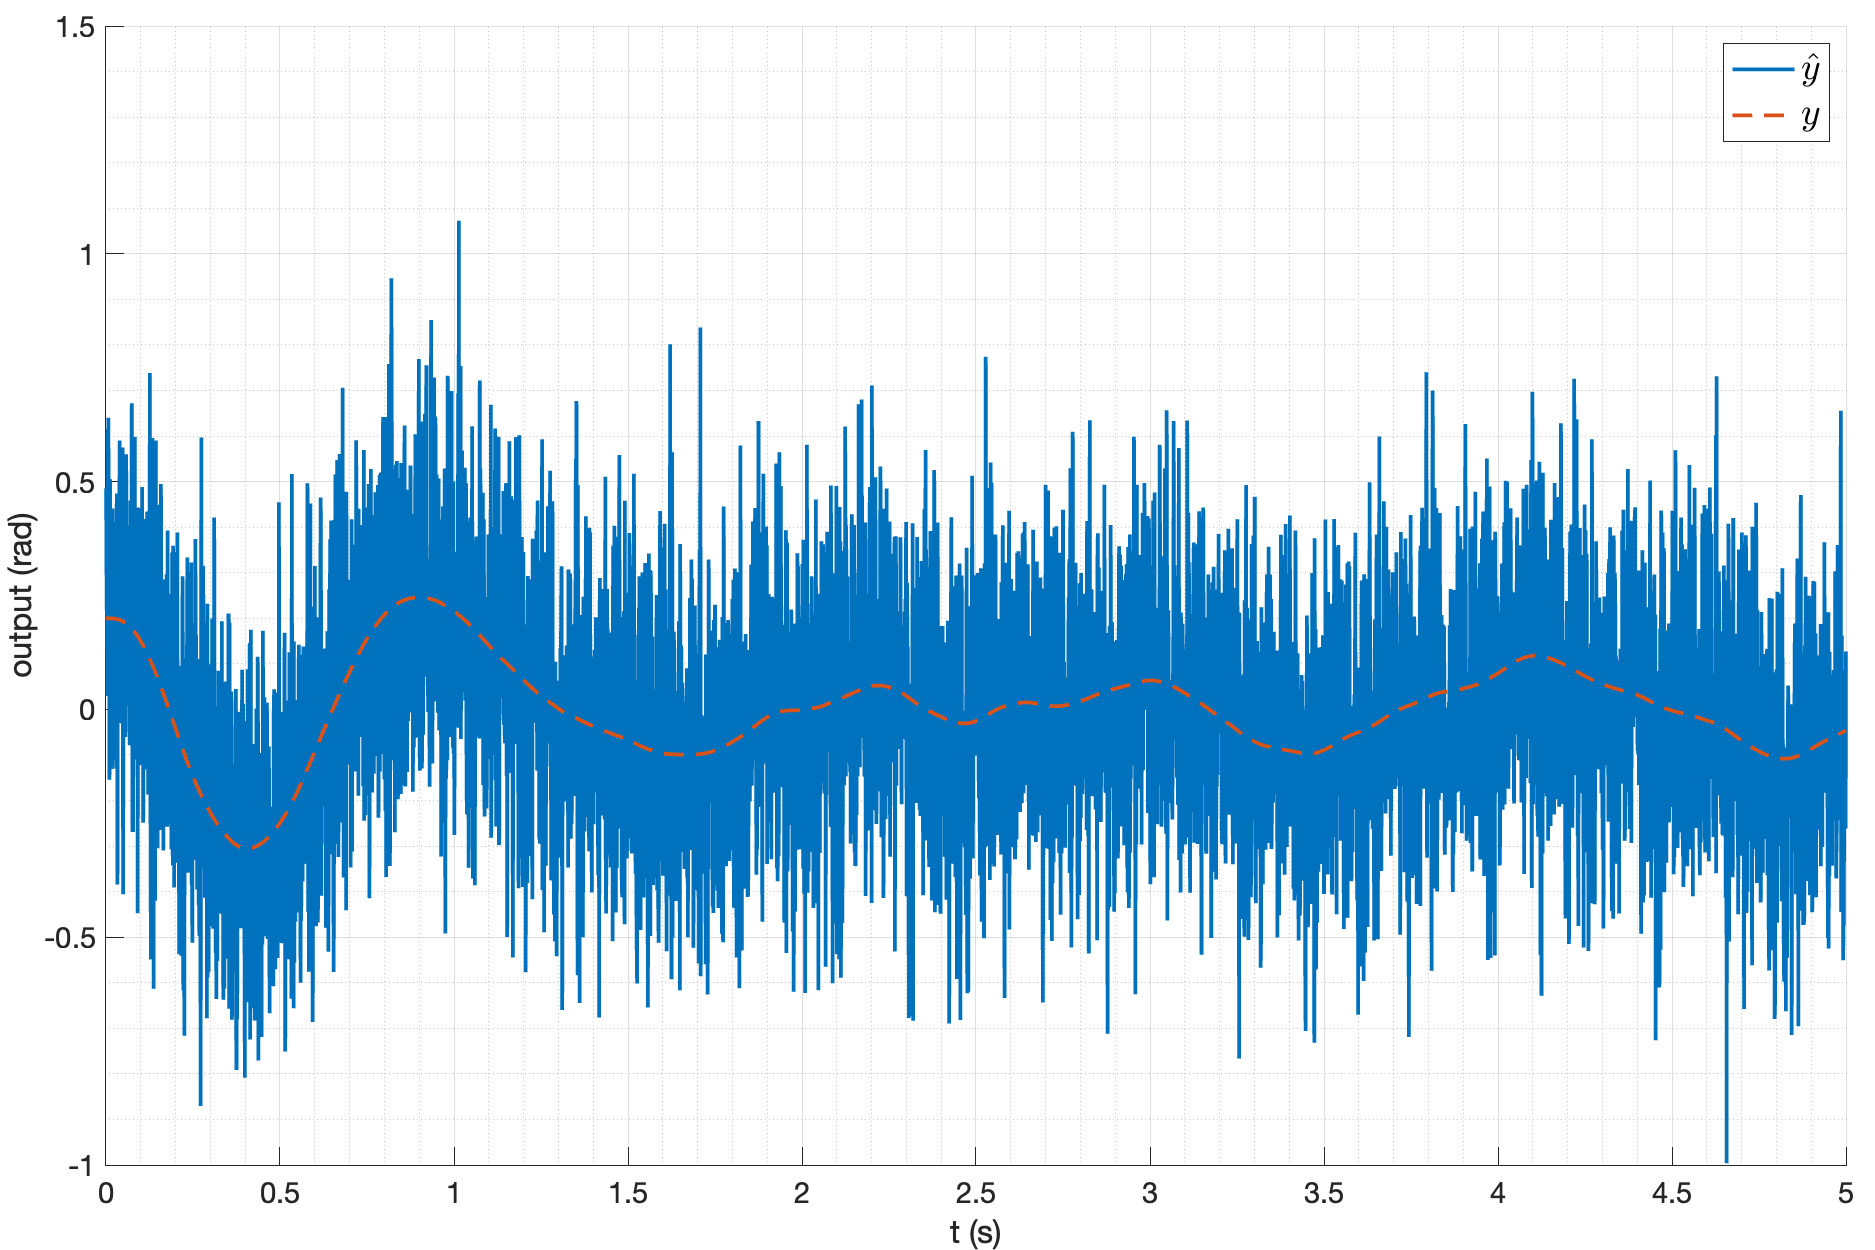
\includegraphics[width=\textwidth]{media/plots/LQG/observer_y2_cmp_1.png}
        \caption{Выход системы с шумом (компонента $y_2$)}
    \end{subfigure}
    \caption{Выход системы с шумом, используемый в качестве входа регулятора}
    \label{fig:lqg_filter_y}
\end{figure}
\FloatBarrier
Сравнение реального состояния системы и оценки состояния фильтром Калмана представлено на рисунке \ref{fig:lqg_filter_cmp} и рисунках 
\ref{fig:lqg_filter_cmp_x1} и \ref{fig:lqg_filter_cmp_ang2}.
\begin{figure}[ht!]
    \centering
    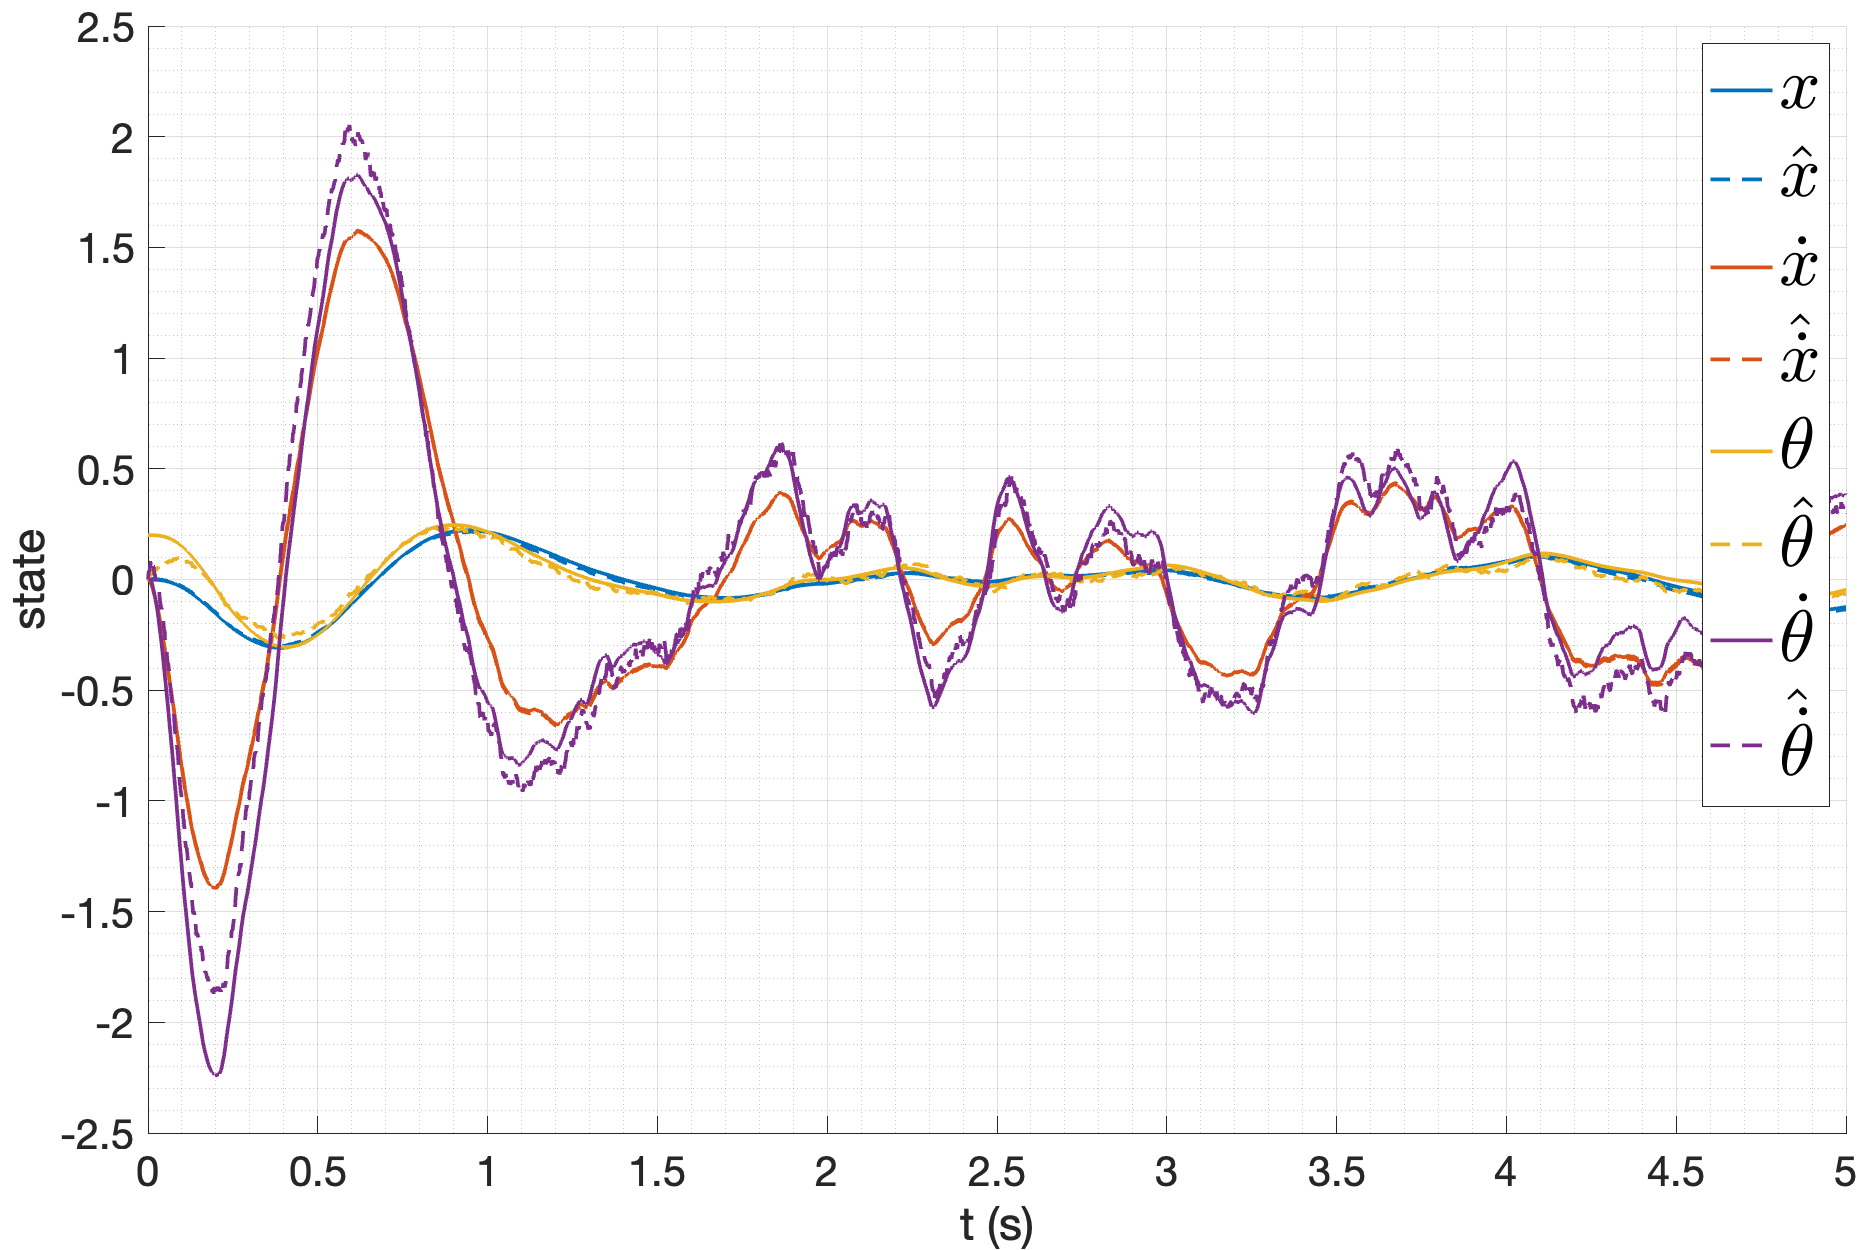
\includegraphics[width=\textwidth]{media/plots/LQG/observer_cmp_1.png}
    \caption{Реальное состояние системы и оценка состояния фильтром Калмана}
    \label{fig:lqg_filter_cmp}
\end{figure}
\begin{figure}[ht!]
    \centering
    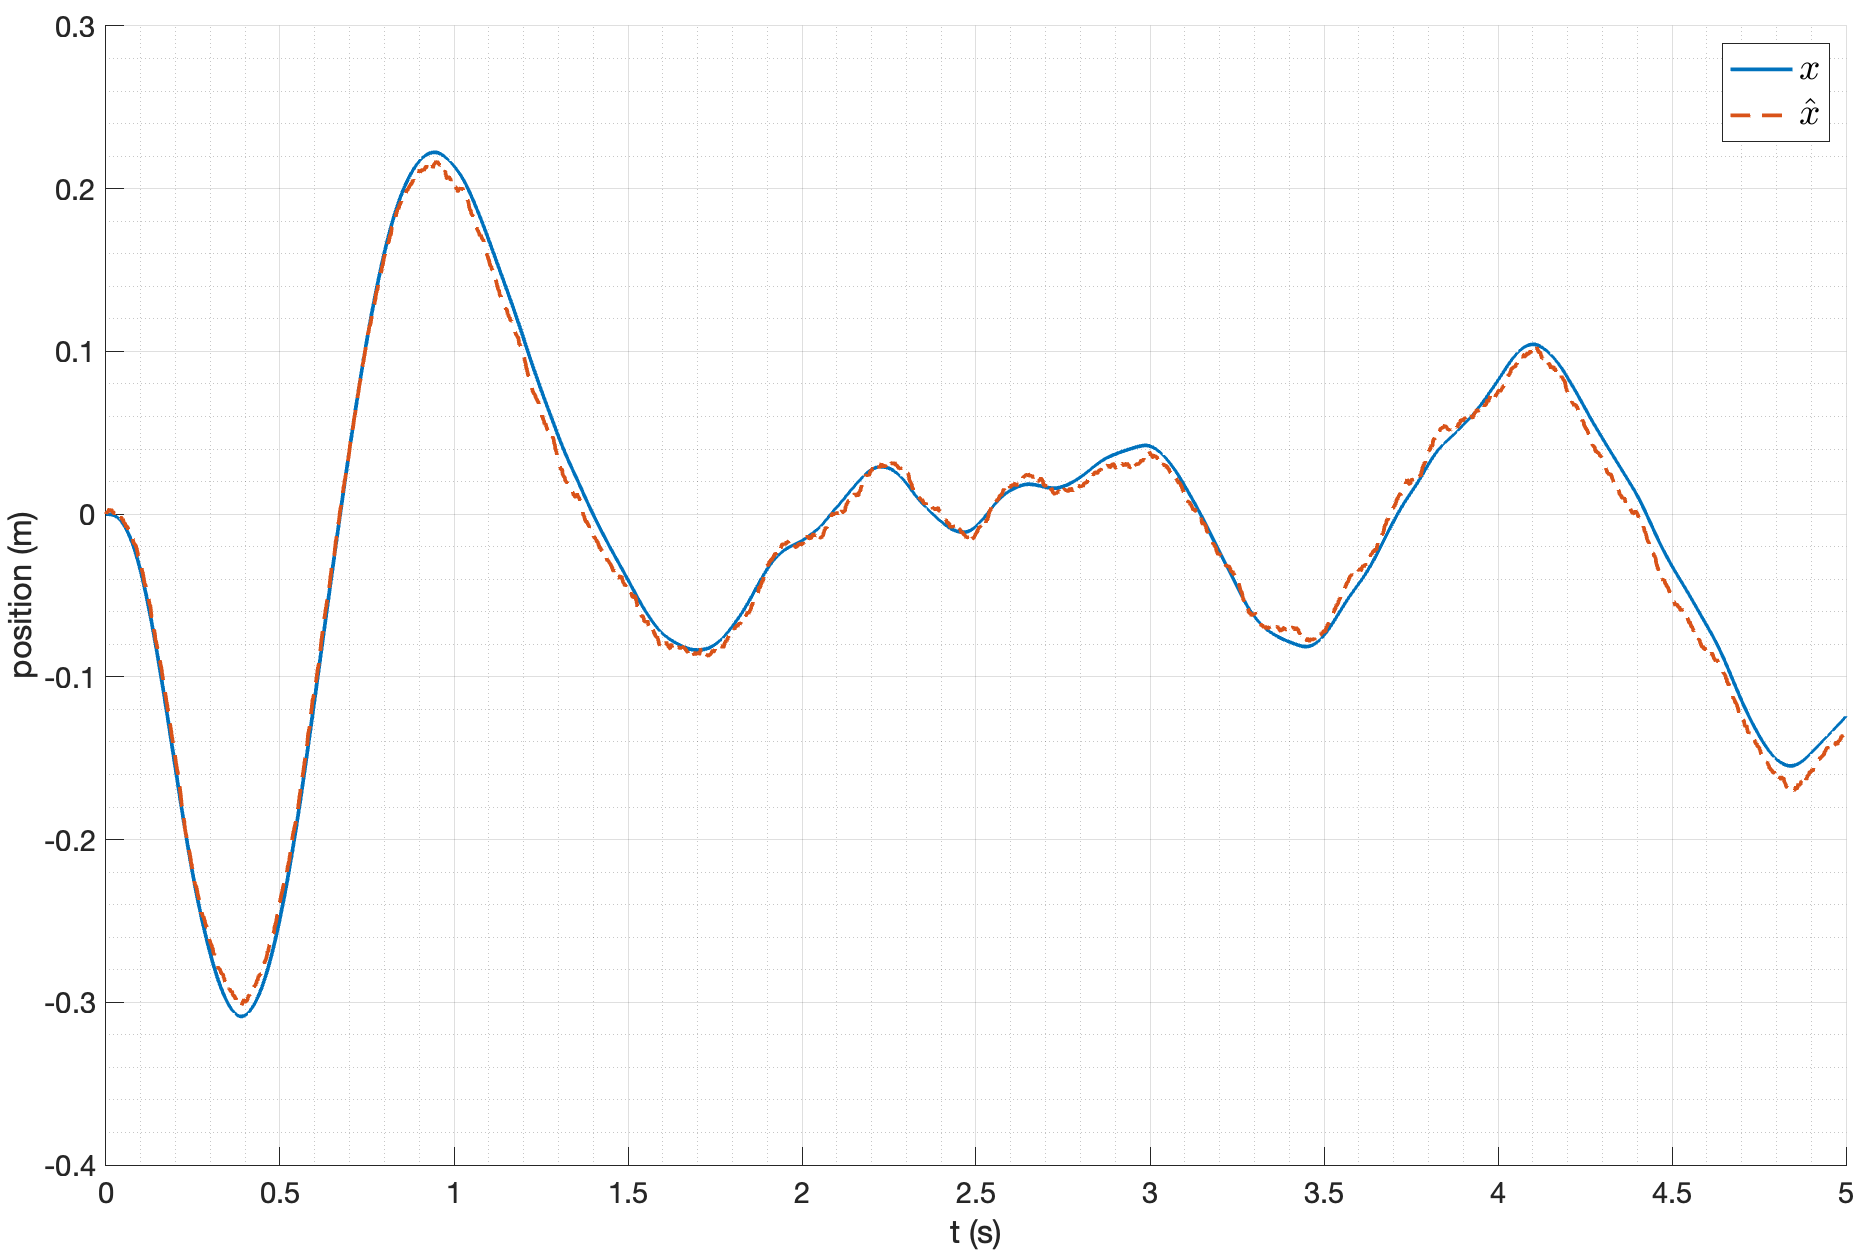
\includegraphics[width=0.8\textwidth]{media/plots/LQG/observer_x_cmp_1.png}
    \caption{Сравнение реального состояния системы и оценки состояния фильтром Калмана (компонента $x$)}
    \label{fig:lqg_filter_cmp_x1} 
\end{figure}
\begin{figure}[ht!]
    \centering
    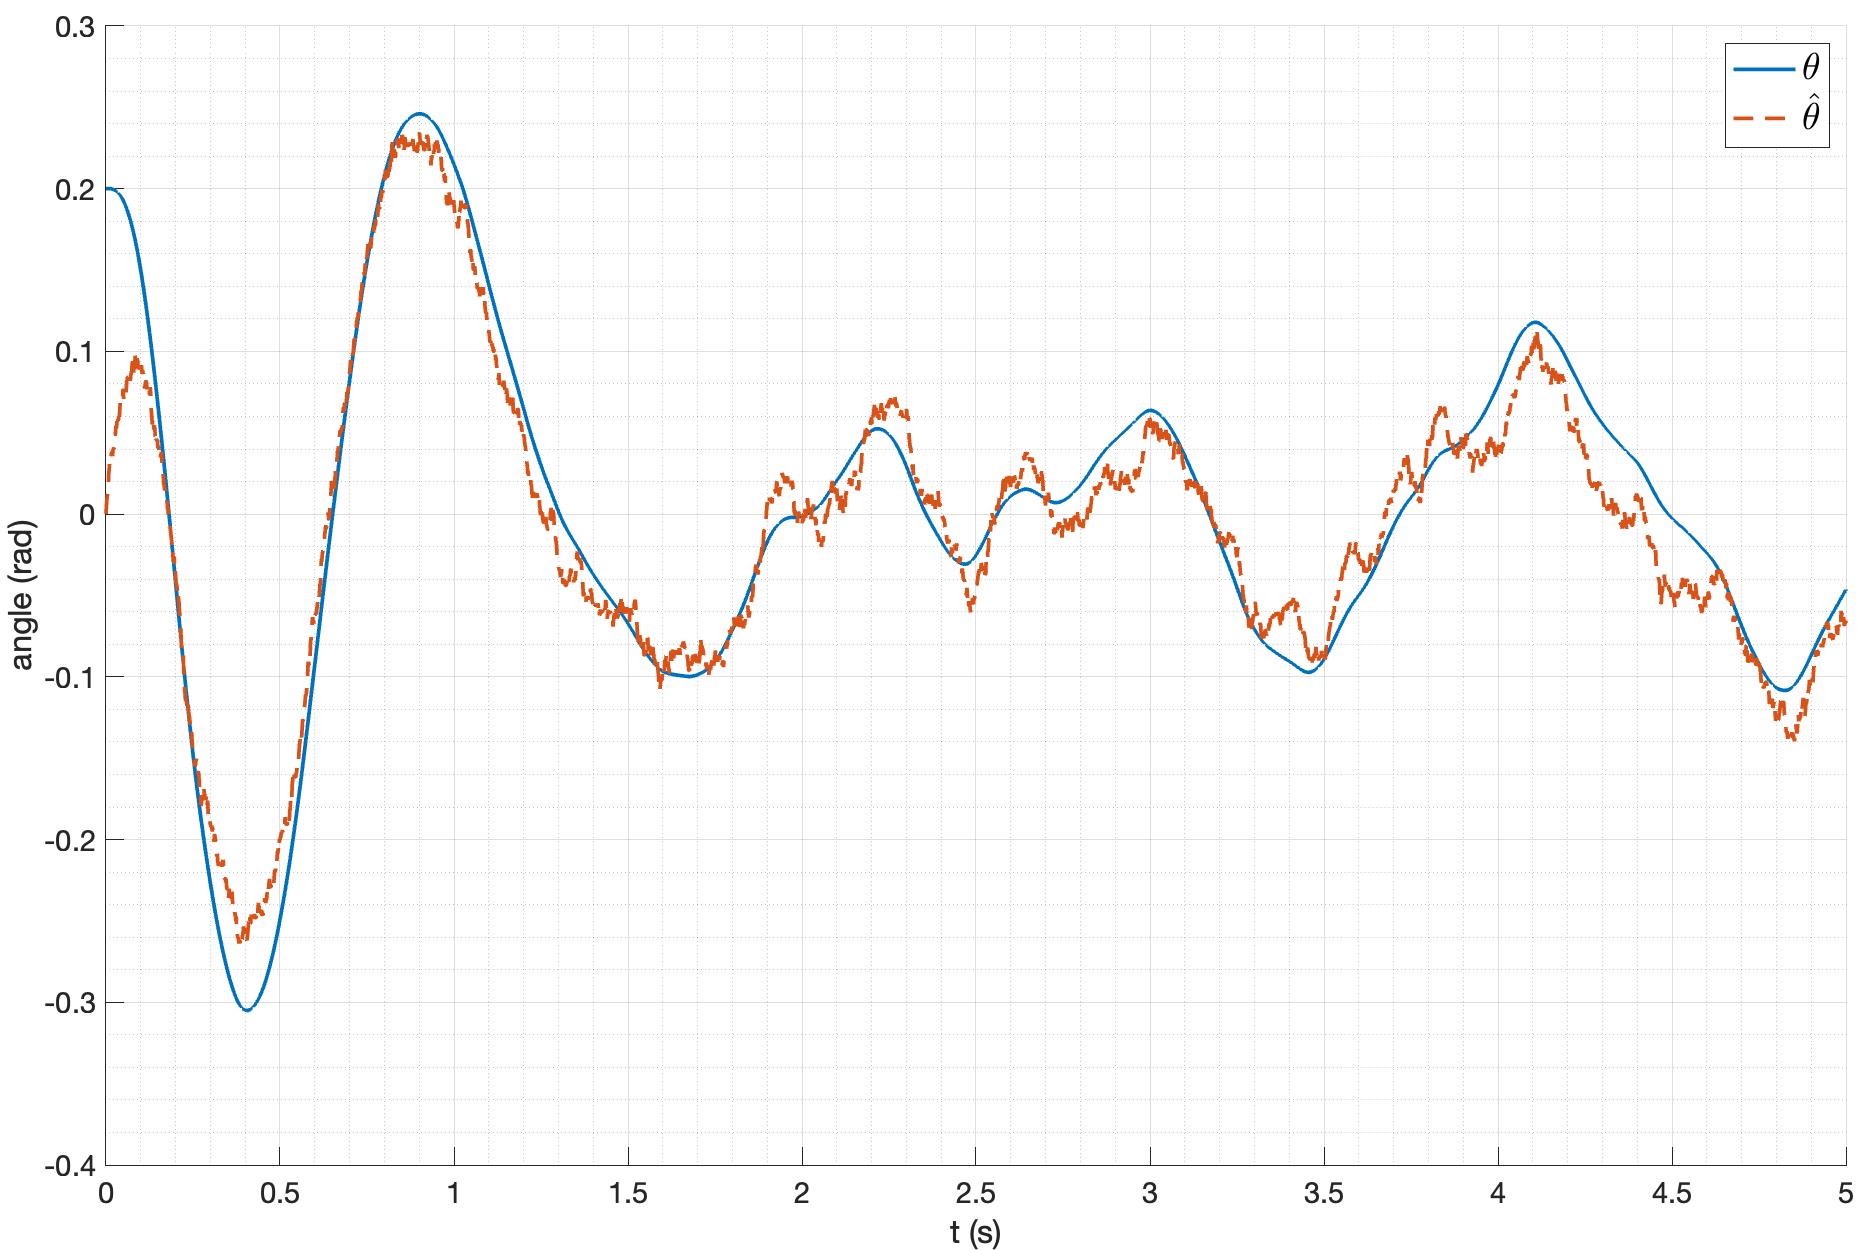
\includegraphics[width=0.8\textwidth]{media/plots/LQG/observer_theta_cmp_1.png}
    \caption{Сравнение реального состояния системы и оценки состояния фильтром Калмана (компонента $\theta$)}
    \label{fig:lqg_filter_cmp_ang2}
\end{figure}

График ошибки оценки состояния фильтром Калмана представлен на рисунке \ref{fig:lqg_filter_err}. 
\begin{figure}[ht!]
    \centering
    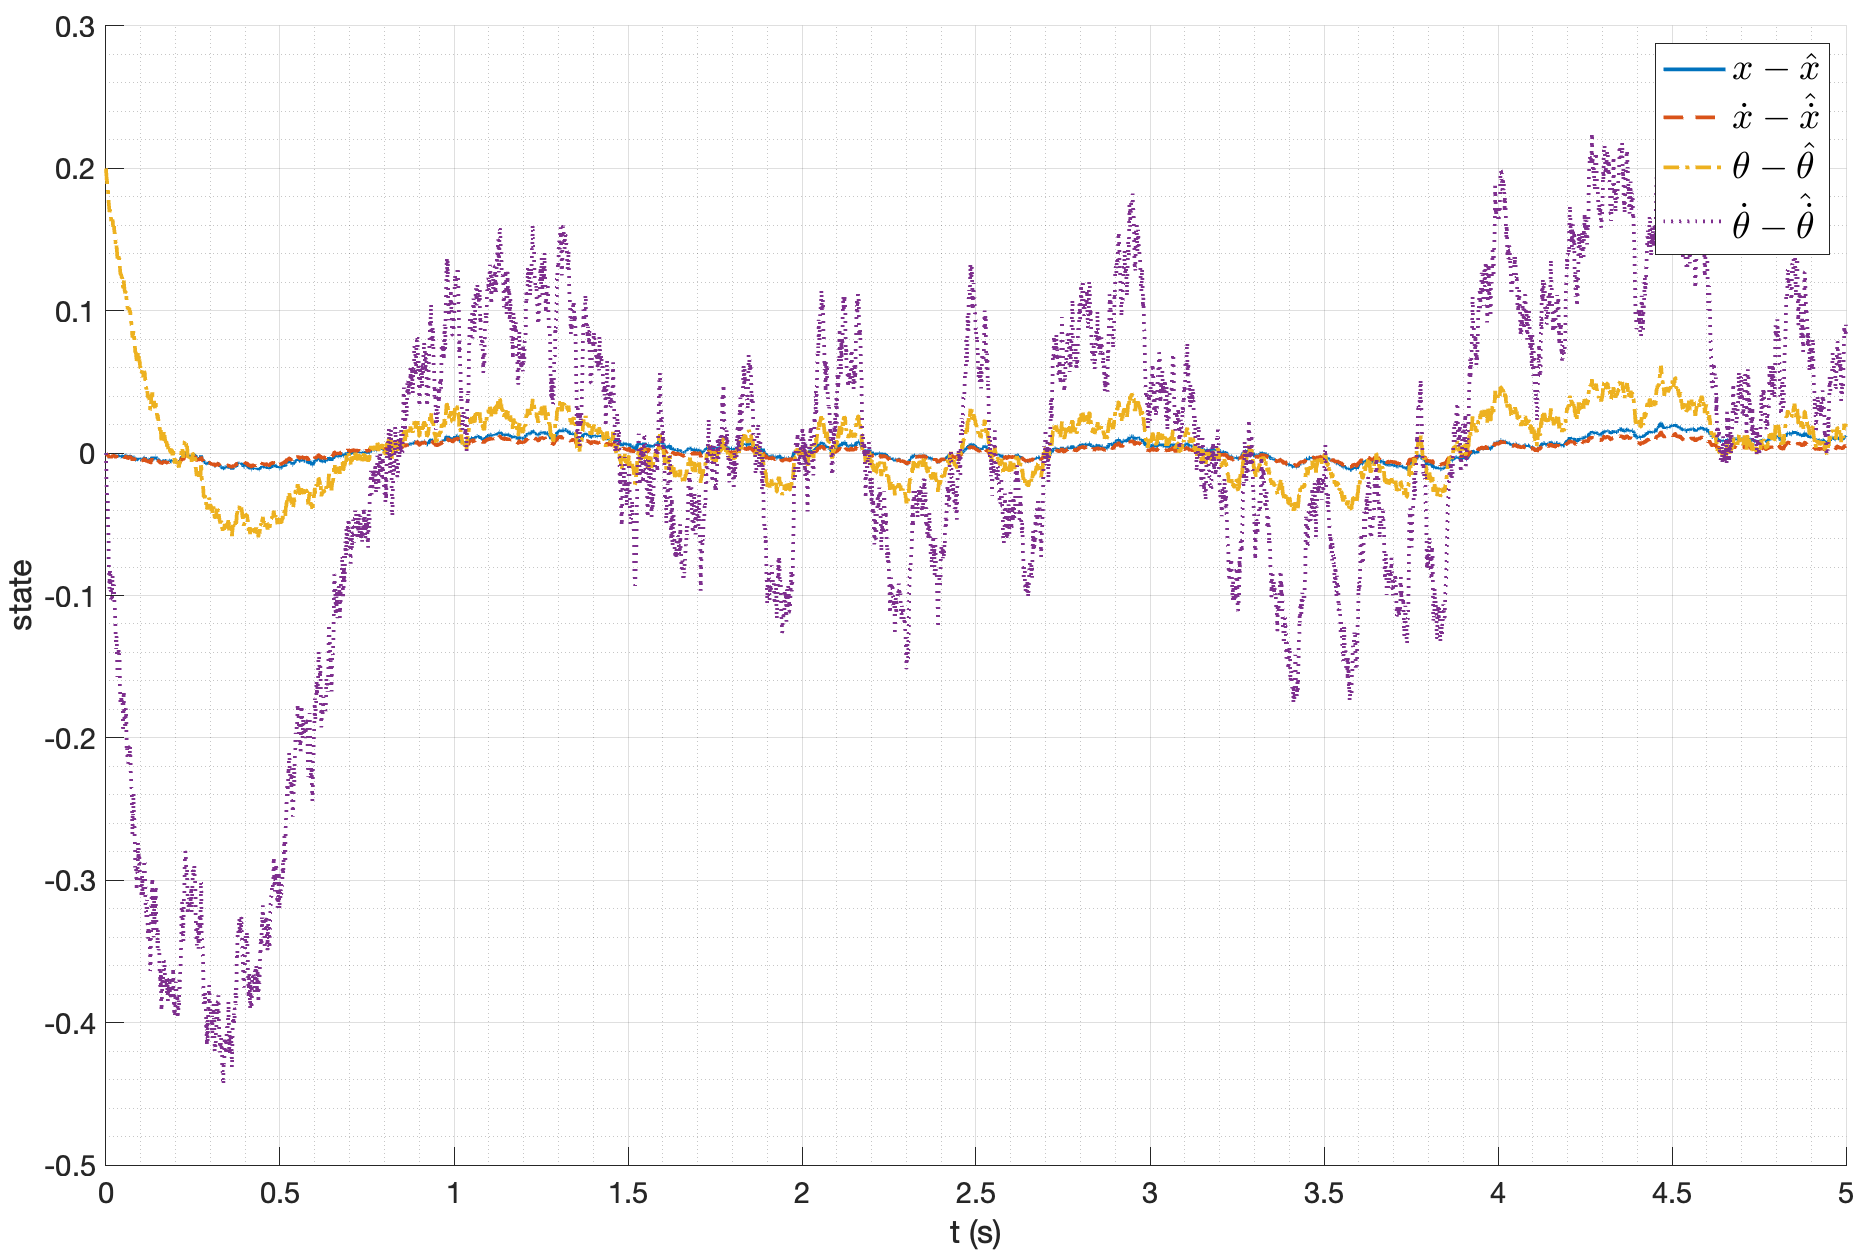
\includegraphics[width=\textwidth]{media/plots/LQG/observer_err_1.png}
    \caption{Оценка ошибки фильтра Калмана}
    \label{fig:lqg_filter_err}
\end{figure}
Видно, что система стабилизируется даже при наличии шума в измерениях. Оценка состояния фильтром Калмана достаточно близка к реальному состоянию системы, 
при этом ошибка колеблется около нуля, что можно объяснить наличием шума в измерениях. Сравнивая зашумленный 
выход системы и оценку состояния фильтром Калмана, можно заметить, что фильтр Калмана позволяет значительно
снизить влияние шума на оценку состояния системы. 

\FloatBarrier
\subsection{LQG для нелинейной модели}
Теперь проведем те же исследования для нелинейной модели системы. Будем использовать LQR регулятор совместно с фильтром Калмана, такие же 
как и для линейной модели. 

Результаты моделирования представлены на рисунке \ref{fig:lqgn_filter}. 
\begin{figure}[ht!]
    \centering
    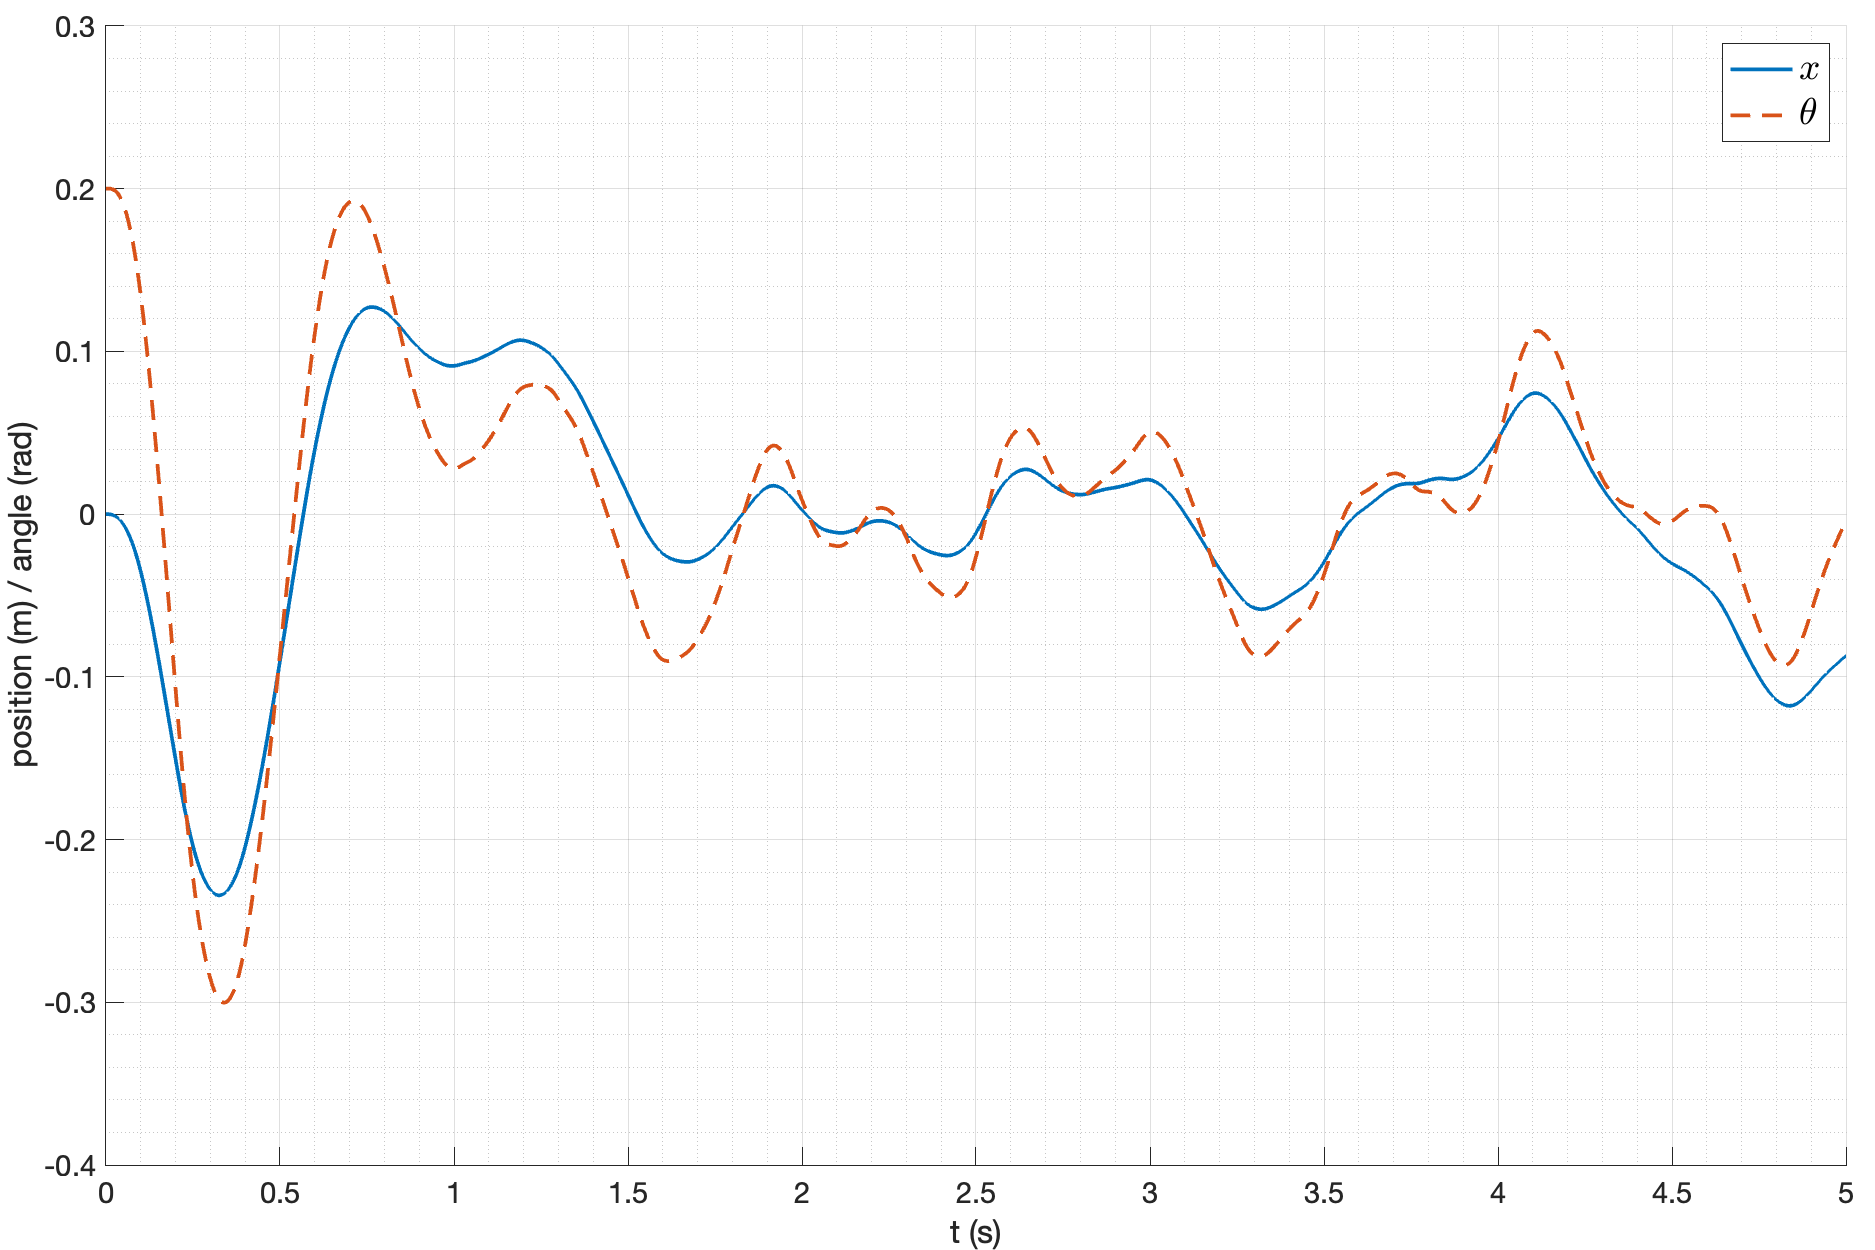
\includegraphics[width=\textwidth]{media/plots/LQGn/out_1.png}
    \caption{Выход системы при использовании LQG регулятора}
    \label{fig:lqgn_filter}
\end{figure}
Вход регулятора (зашумленный выход системы) представлен на рисунке \ref{fig:lqgn_filter_y}. 
\begin{figure}[ht!]
    \begin{subfigure}[b]{0.45\textwidth}
        \centering
        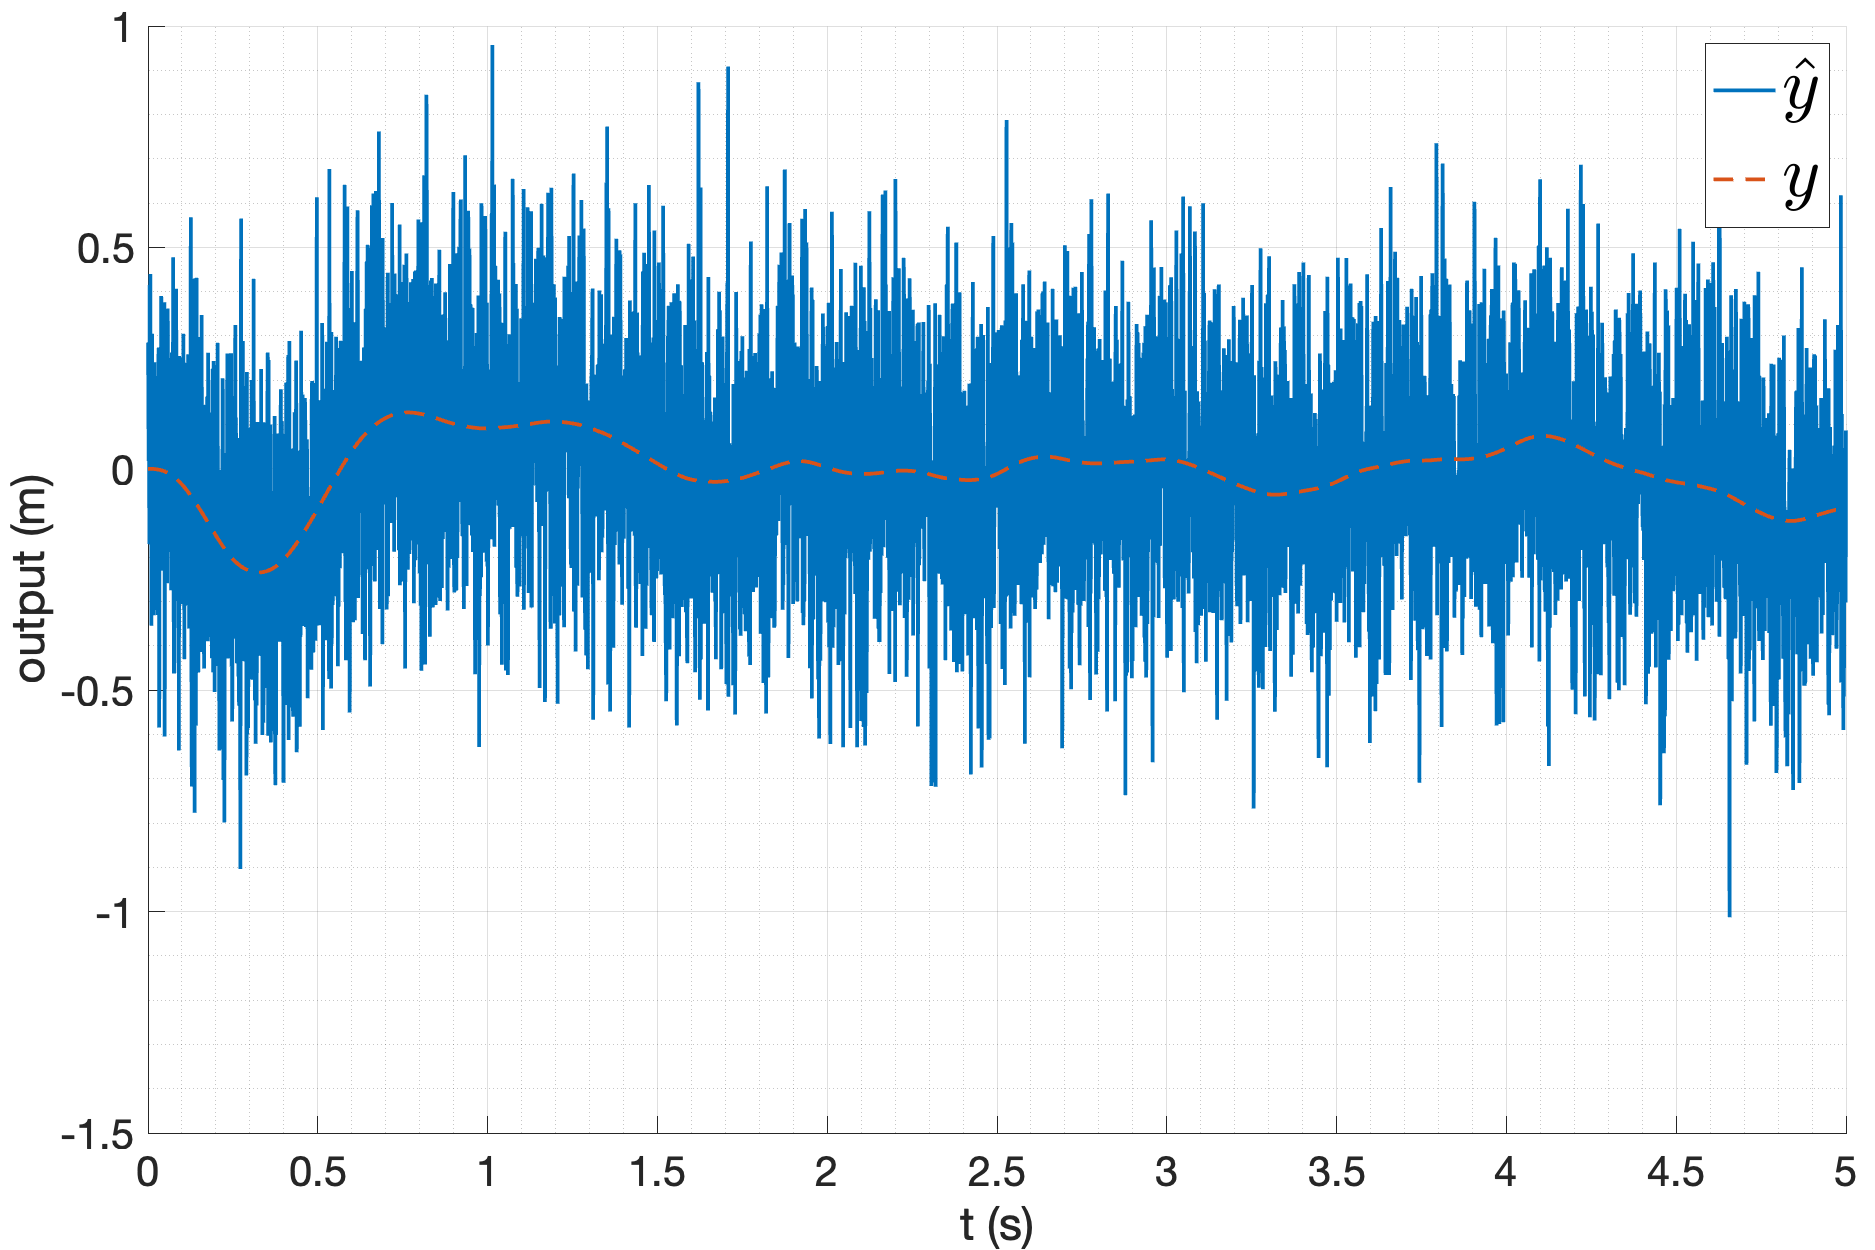
\includegraphics[width=\textwidth]{media/plots/LQGn/observer_y1_cmp_1.png}
        \caption{Выход системы с шумом (компонента $y_1$)}
    \end{subfigure}
    \begin{subfigure}[b]{0.45\textwidth}
        \centering
        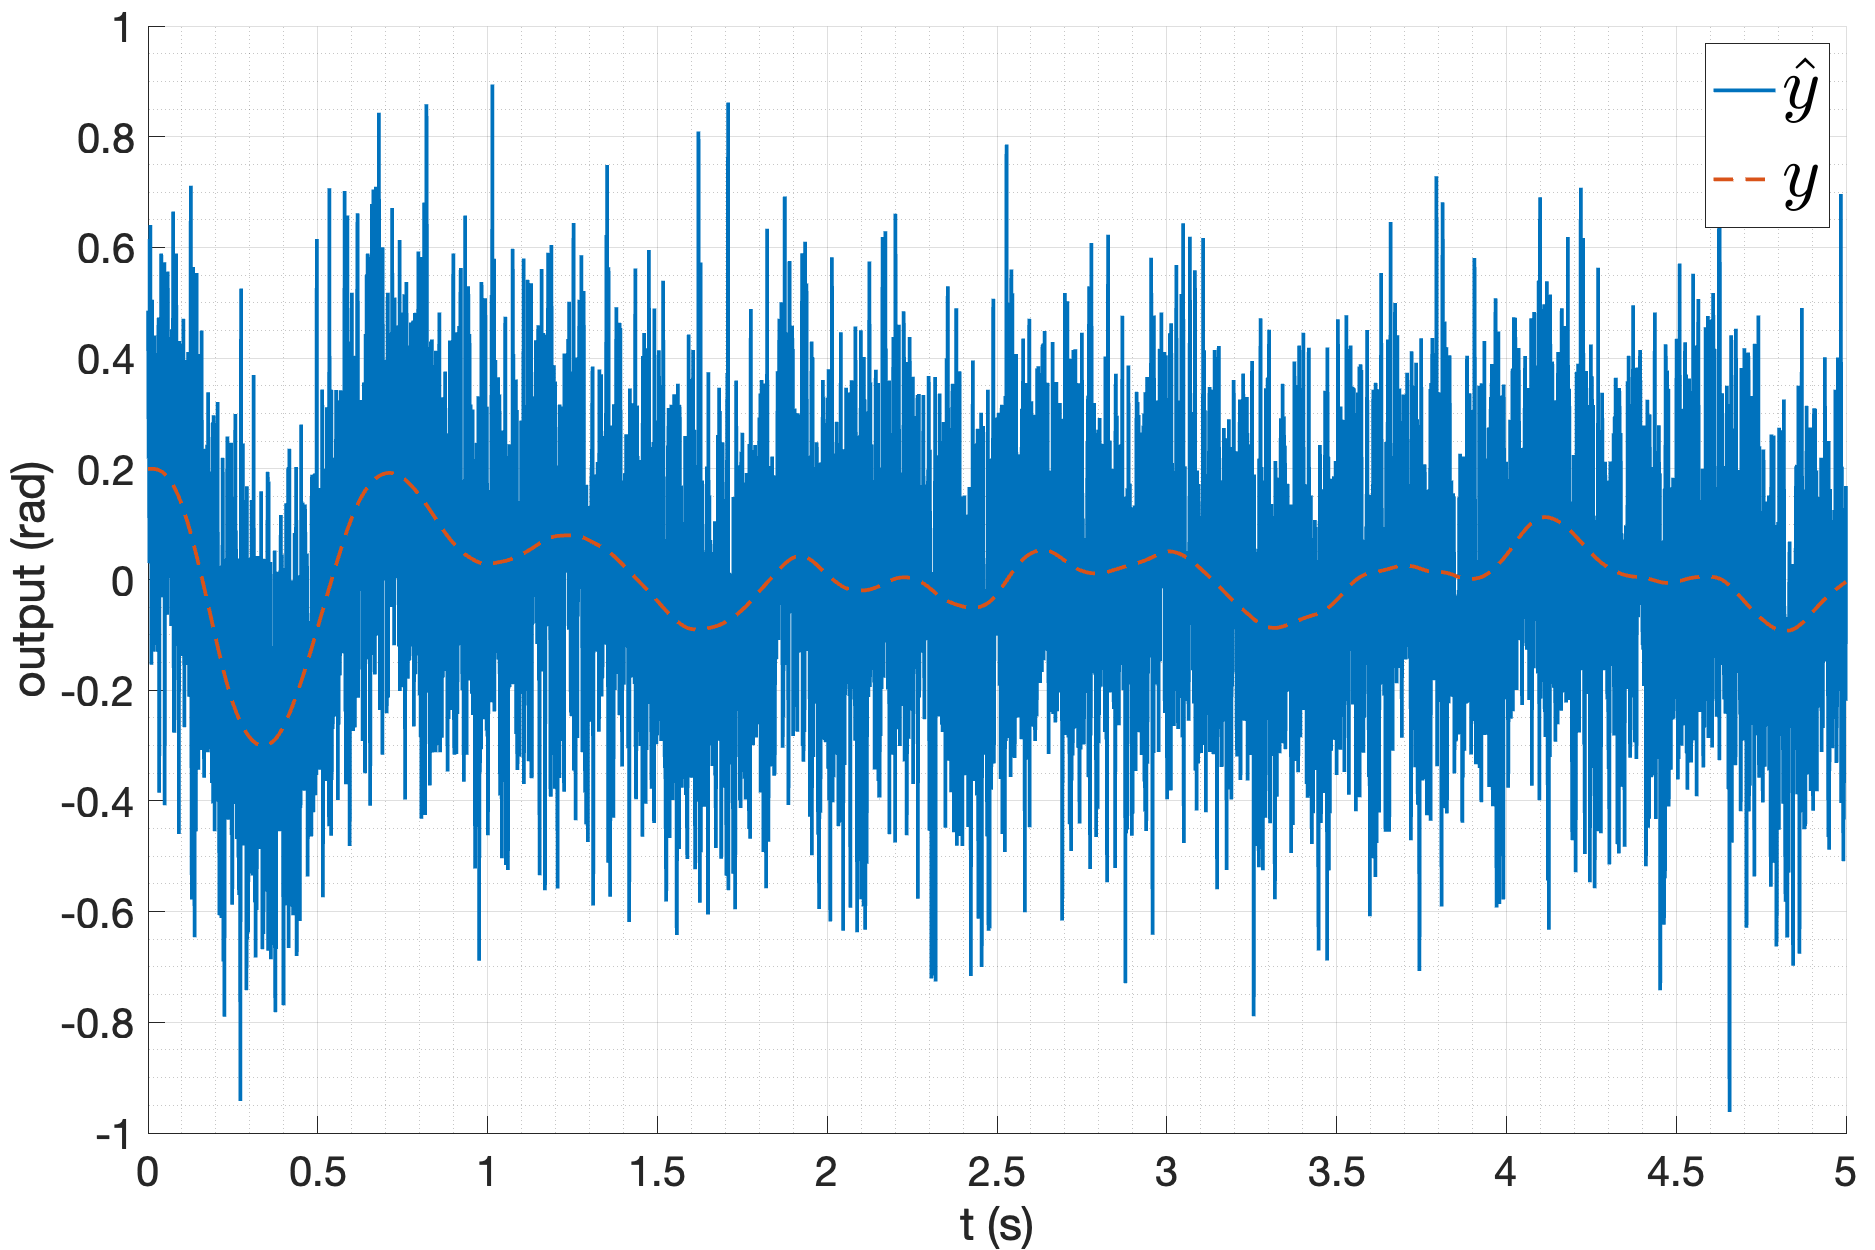
\includegraphics[width=\textwidth]{media/plots/LQGn/observer_y2_cmp_1.png}
        \caption{Выход системы с шумом (компонента $y_2$)}
    \end{subfigure}
    \caption{Выход системы с шумом, используемый в качестве входа регулятора}
    \label{fig:lqgn_filter_y}
\end{figure}
\FloatBarrier
Сравнение реального состояния системы и оценки состояния фильтром Калмана представлено на рисунке \ref{fig:lqgn_filter_cmp} и рисунках 
\ref{fig:lqgn_filter_cmp_x1} и \ref{fig:lqgn_filter_cmp_ang2}.
\begin{figure}[ht!]
    \centering
    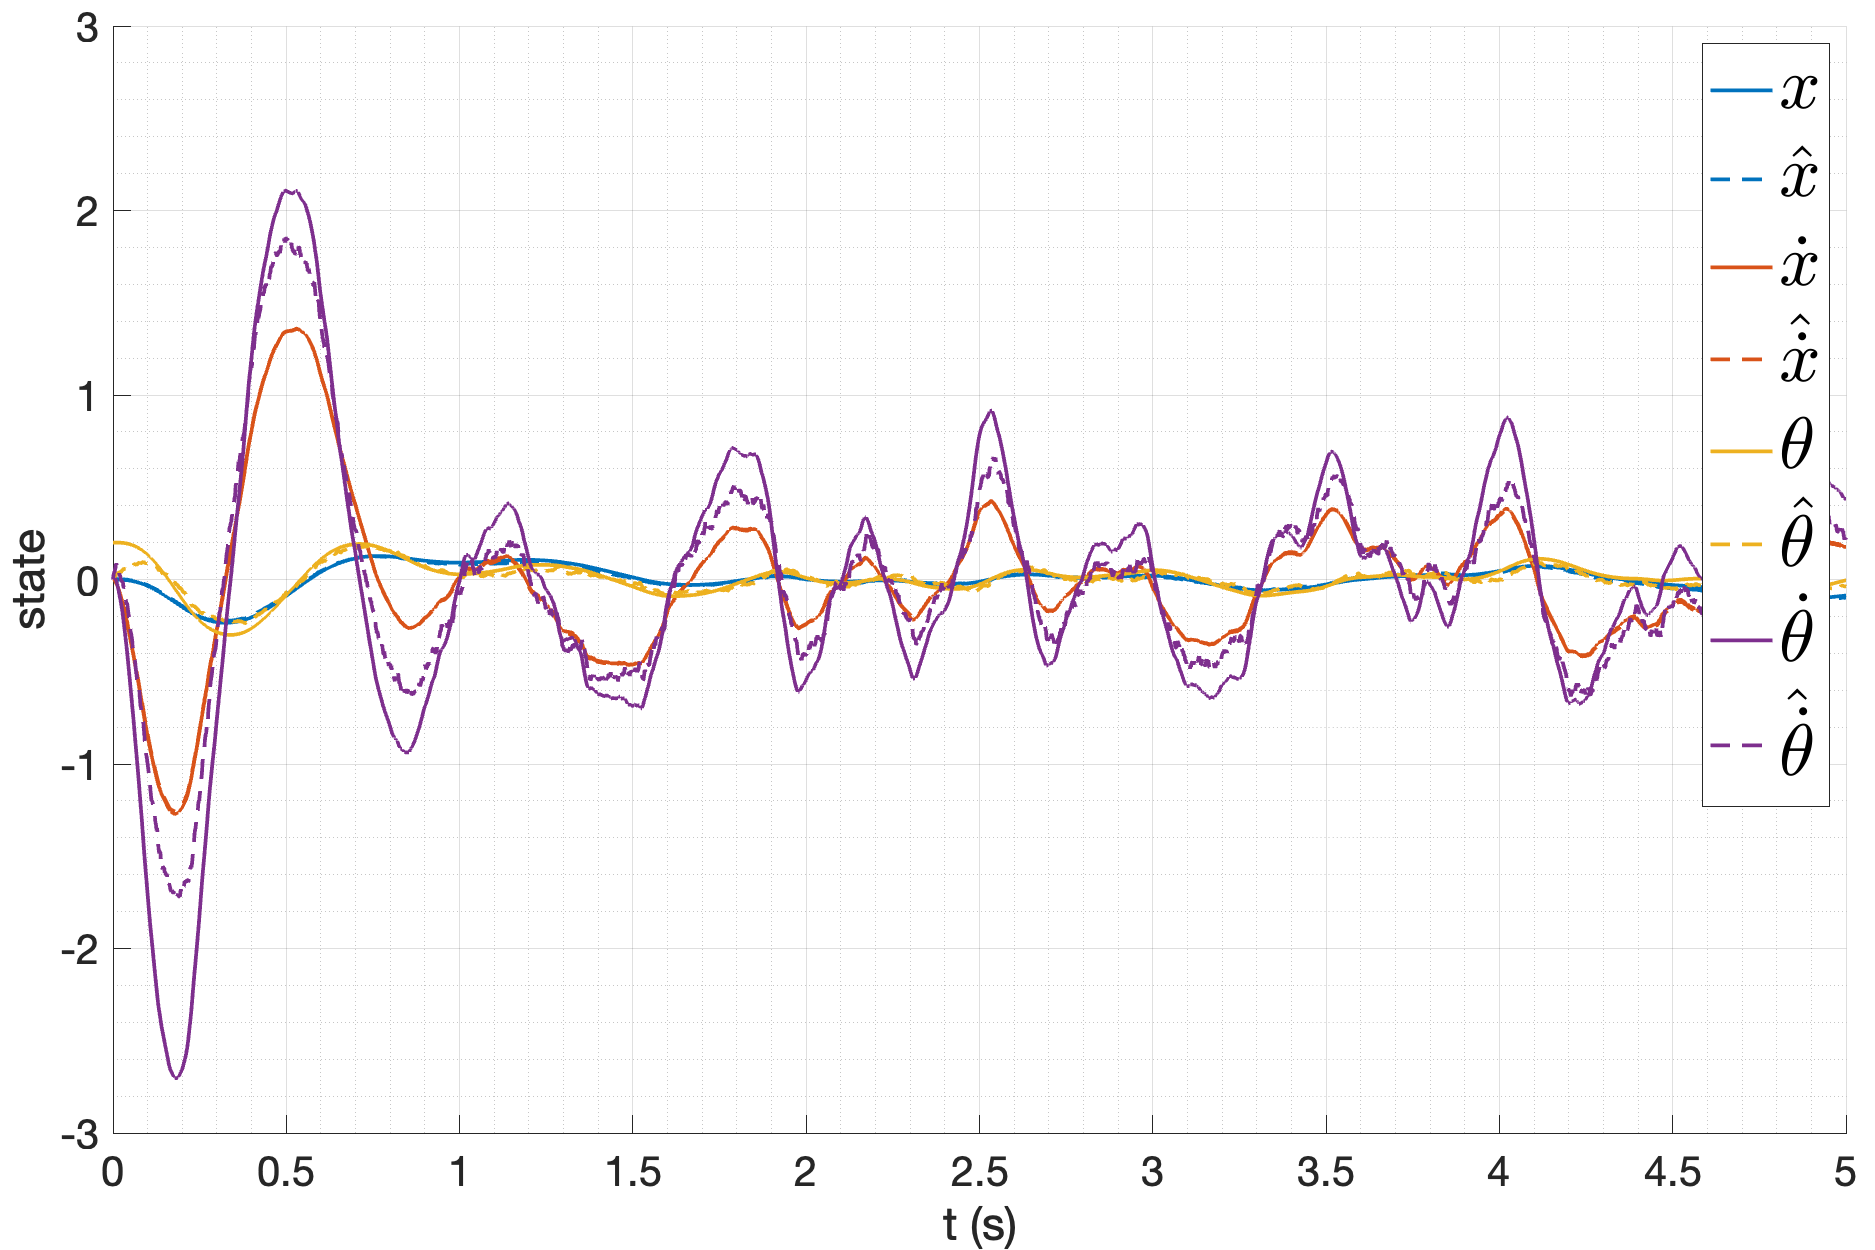
\includegraphics[width=\textwidth]{media/plots/LQGn/observer_cmp_1.png}
    \caption{Реальное состояние системы и оценка состояния фильтром Калмана}
    \label{fig:lqgn_filter_cmp}
\end{figure}
\begin{figure}[ht!]
    \centering
    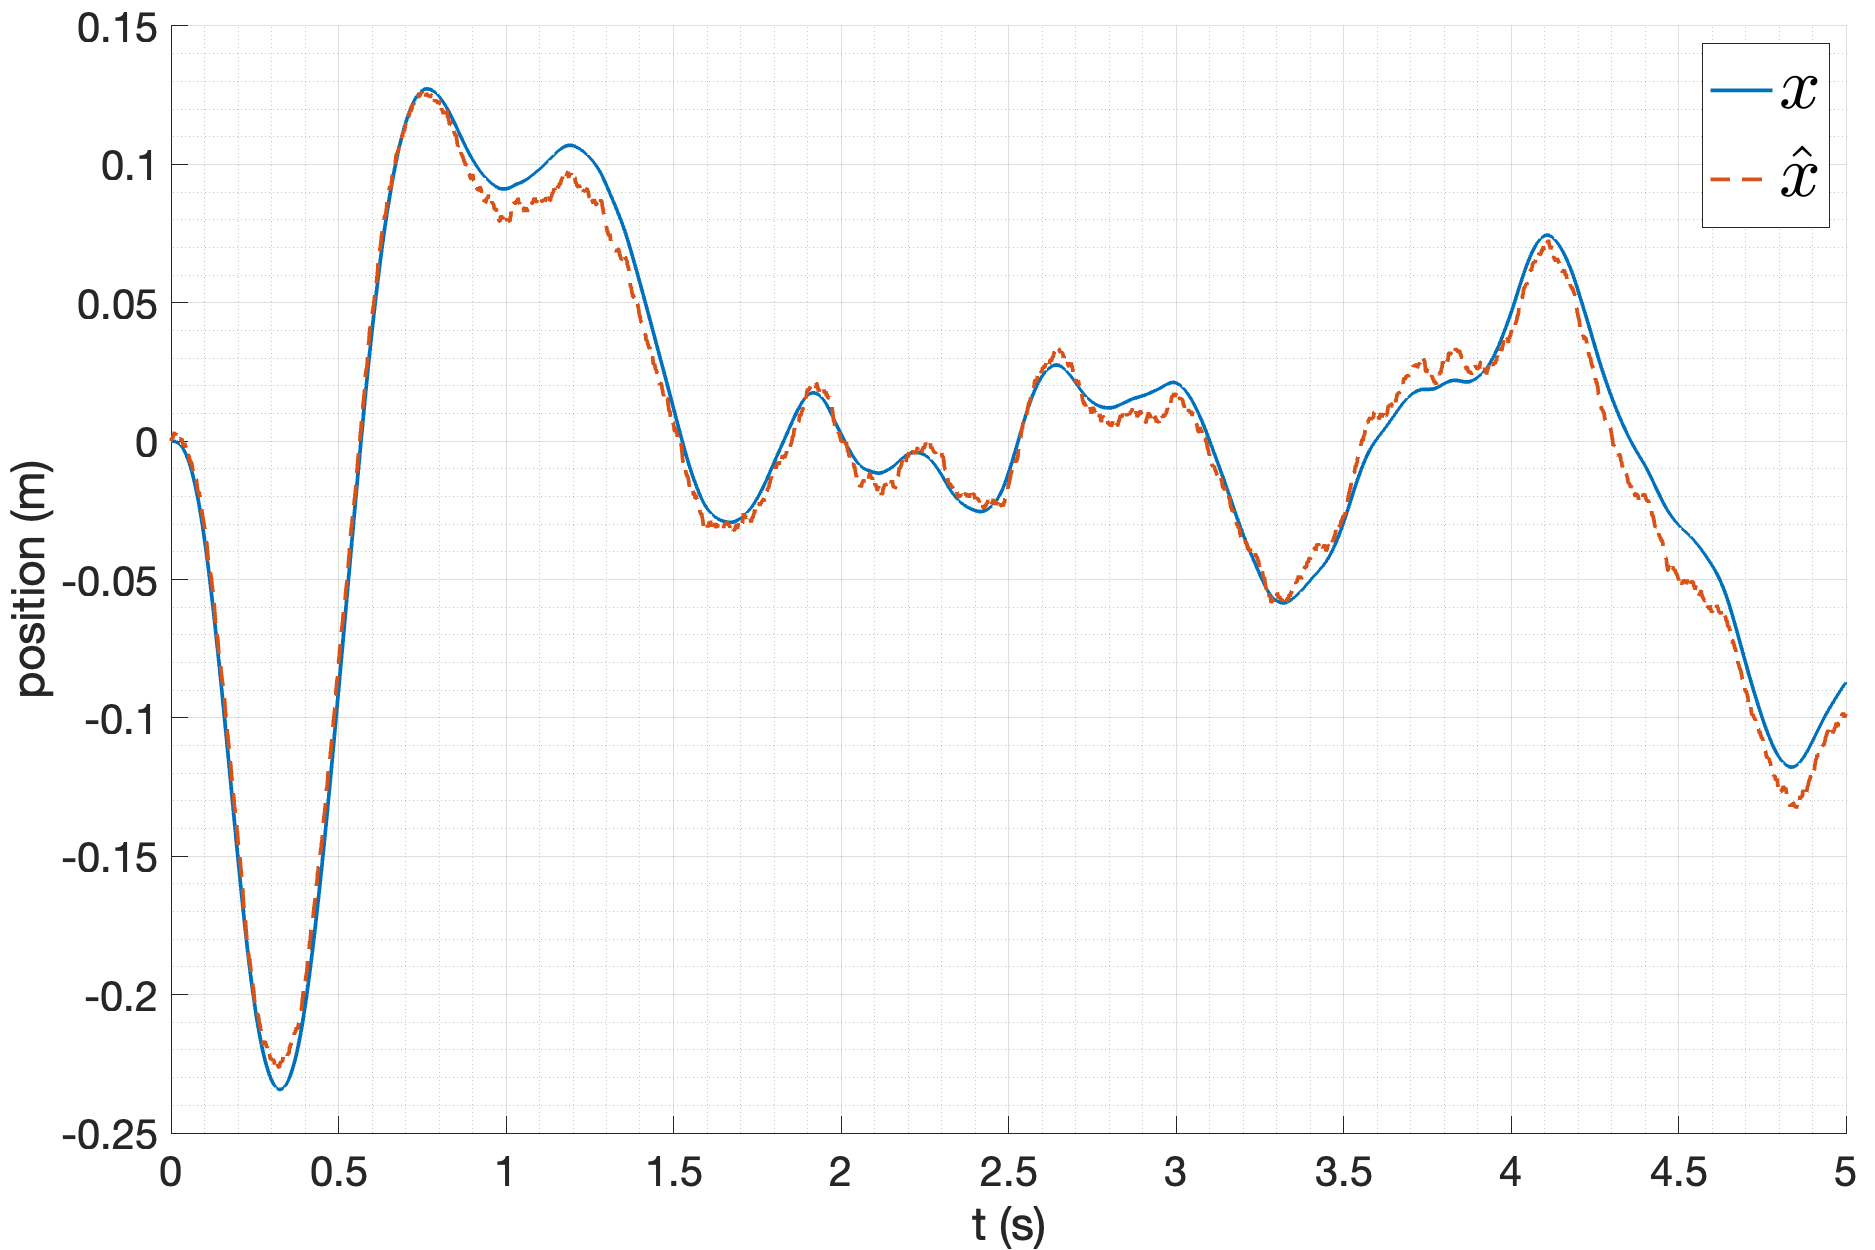
\includegraphics[width=0.8\textwidth]{media/plots/LQGn/observer_x_cmp_1.png}
    \caption{Сравнение реального состояния системы и оценки состояния фильтром Калмана (компонента $x$)}
    \label{fig:lqgn_filter_cmp_x1} 
\end{figure}
\begin{figure}[ht!]
    \centering
    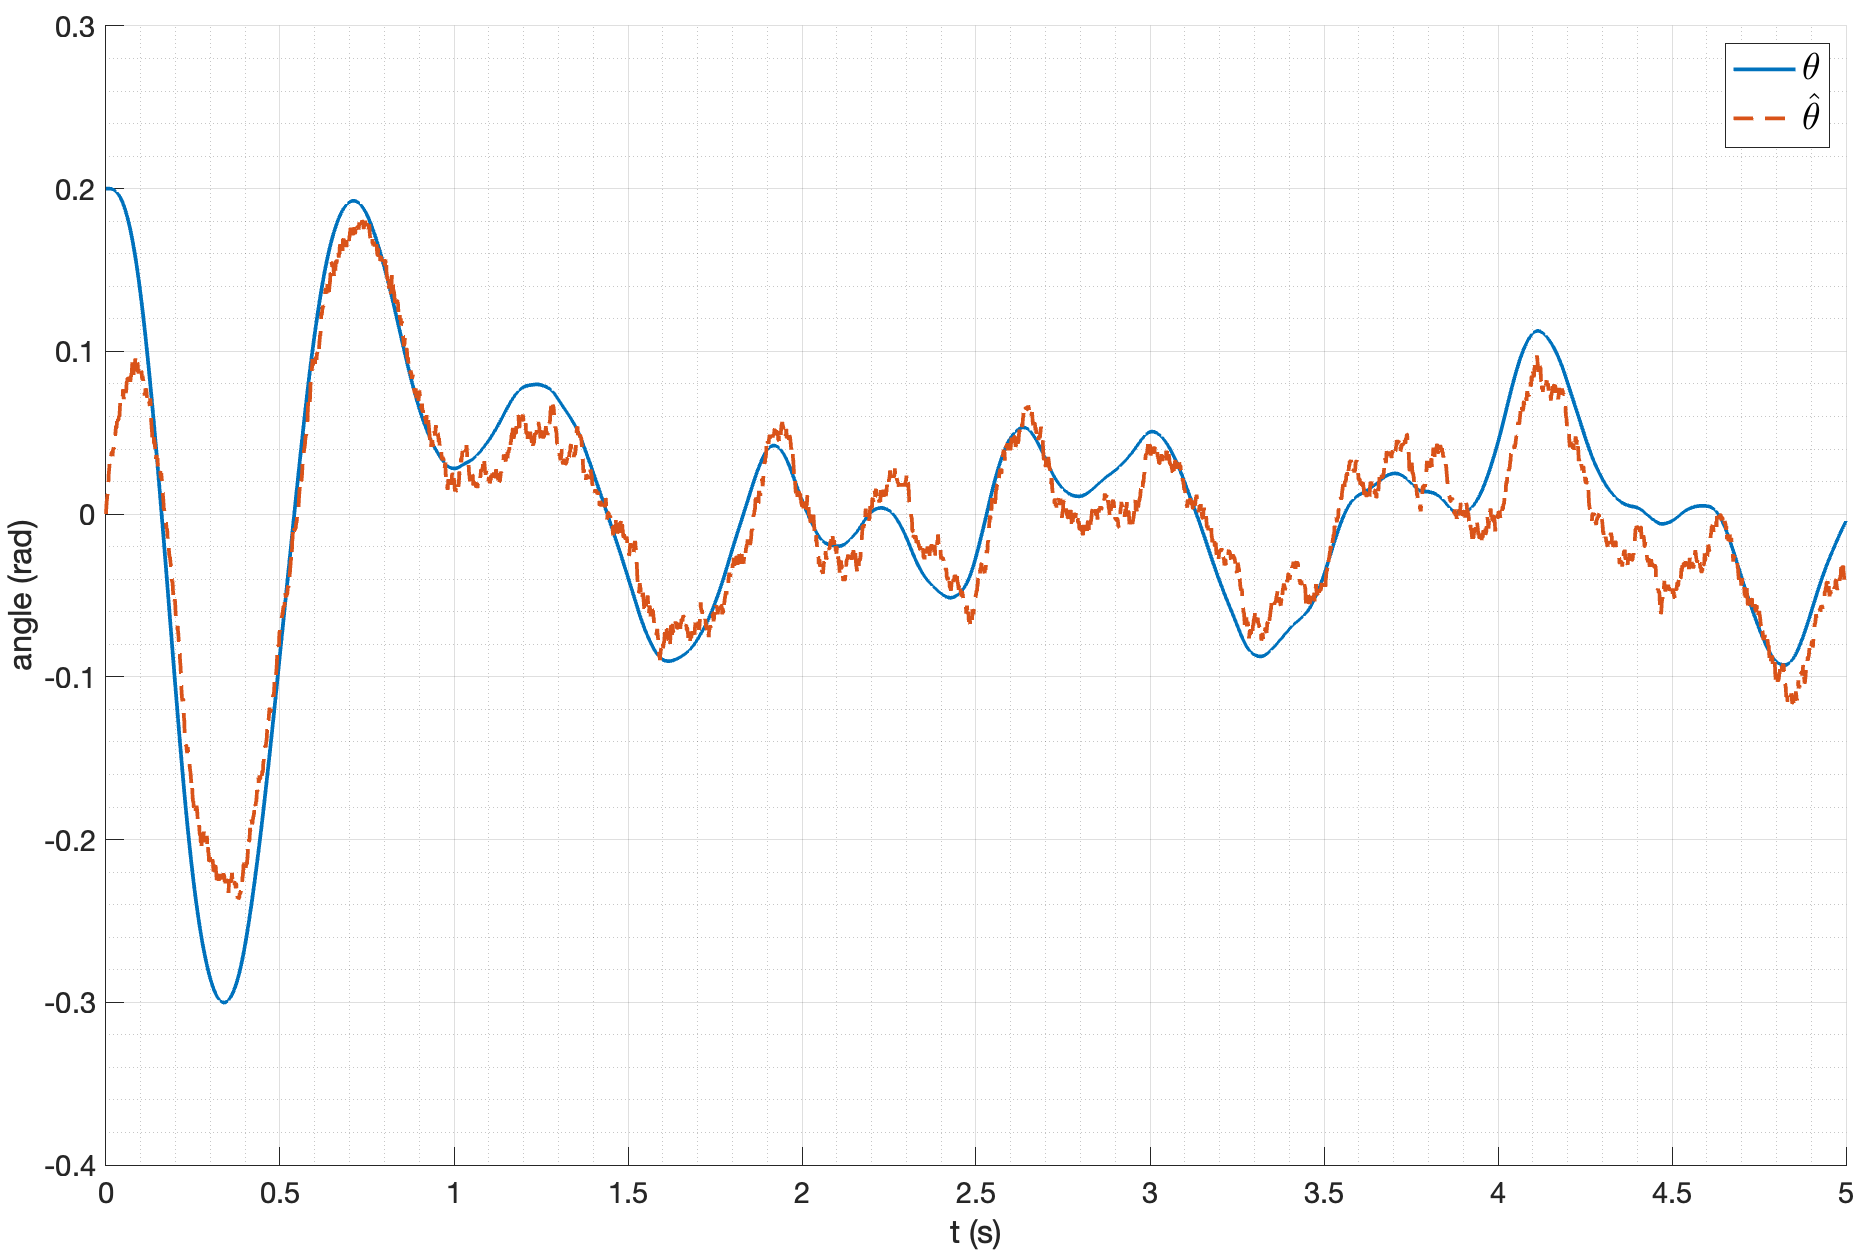
\includegraphics[width=0.8\textwidth]{media/plots/LQGn/observer_theta_cmp_1.png}
    \caption{Сравнение реального состояния системы и оценки состояния фильтром Калмана (компонента $\theta$)}
    \label{fig:lqgn_filter_cmp_ang2}
\end{figure}

График ошибки оценки состояния фильтром Калмана представлен на рисунке \ref{fig:lqgn_filter_err}. 
\begin{figure}[ht!]
    \centering
    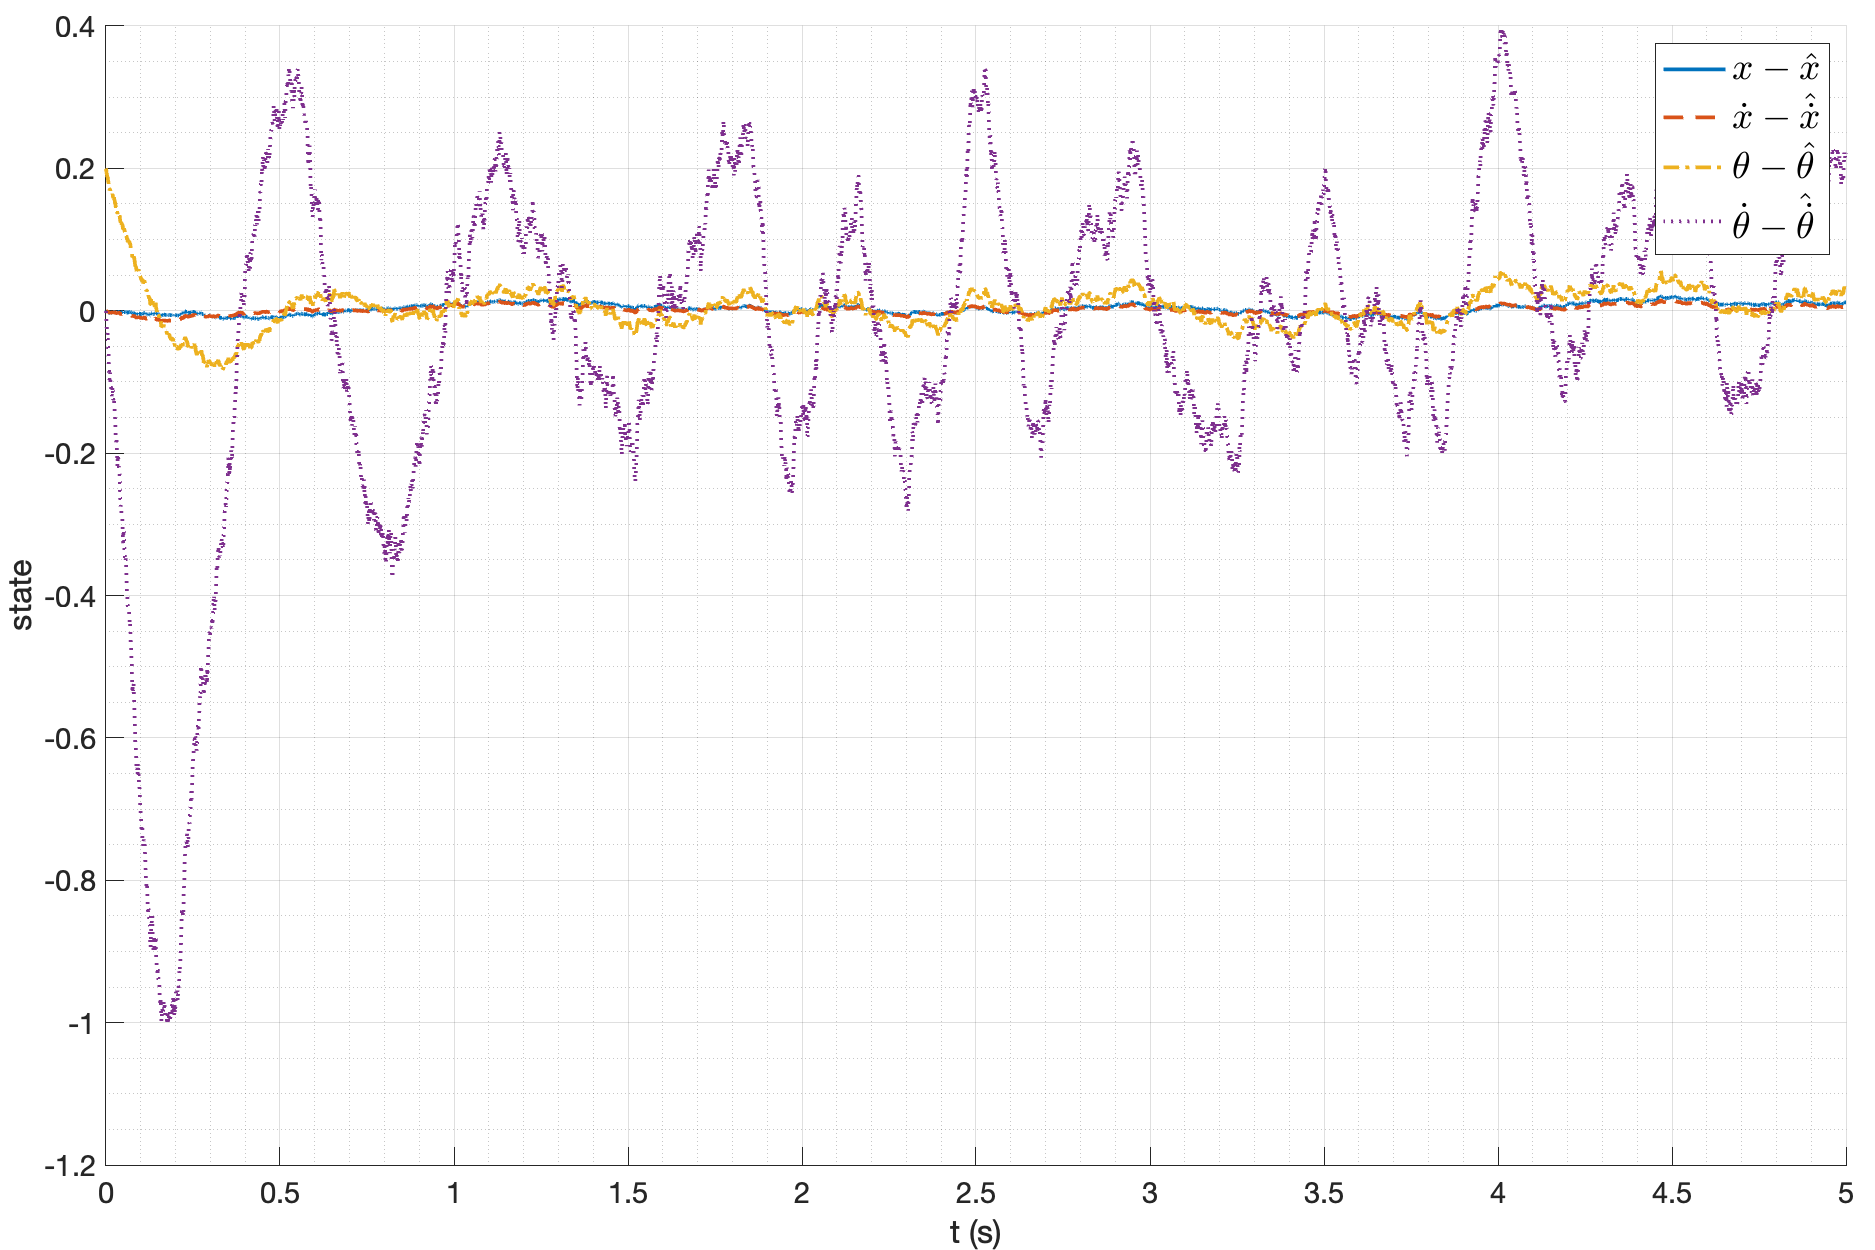
\includegraphics[width=\textwidth]{media/plots/LQGn/observer_err_1.png}
    \caption{Оценка ошибки фильтра Калмана}
    \label{fig:lqgn_filter_err}
\end{figure}

Как и в случае линейной модели, видно, что система стабилизируется даже при наличии шума в измерениях. При этом ошибка 
оценки также колеблется около нуля, но уже с большей амплитудой, что связано с тем, что линейная модель 
системы, на основе которой был синтезирован регулятор, не является точной моделью реальной системы. 